% !TEX root = ../main.tex

\chapter{绪论}
近些年来, 由于互联网的普及, 计算机技术的发展和各种社交网络的兴起, 视频和图片数据以爆炸性的速度快速增长。如何对海量的图像数据进行处理以及分析促进了一系列的计算机视觉技术的飞速发展,图像检索技术是其中一个核心研究方向。早期基于文本的图像检索极大依赖于标注者的主观判断的标签,检索效率以及性能低下的同时需要耗费大量的人力资源, 难以应用于海量的互联网图像数据检索中。基于内容的的图像检索(Content Based Image Retrieval, CBIR)通过算法自动提取图像的视觉特征来衡量图片之间的相似度, 从而实现在数据库中进行图像检索的目的,极大的节省了人工标注耗费的人力、物力和财力。为了提高检索速度以及降低存储开销,哈希编码以及量化编码方法被广泛应用到了图像检索领域,成为解决超大规模图像检索问题的重要解决方案。 本章重点介绍大规模图像检索算法的研究背景以及意义,概要的介绍了图像检索算法发展历史, 详细介绍了基于深度哈希的大规模的图像检索算法。 本章最后介绍了这篇论文的章节安排以及概括介绍每个章节包含的主要内容。
\section{本研究的背景及意义}
在大数据、移动互联网、计算机技术、传感器技术、云计算等前沿技术的发展以及经济社会急速发展的需求下,人工智能(Artificial Intelligence)作为被视为驱动新一轮产业变革的技术受到了世界各国的广泛关注。 广义的人工智能\cite{russell2010artificial} 包含对大数据的处理分析,自动推理能力,学习能力,以及解决问题的能力。而对以往存储的大数据信息的检索是后续学习与分析的基石,而图像检索便是其中关键的一部分。 \par
基于内容图像检索自从1990年代以来便受到了计算机视觉研究人员广泛的探索~\cite{zhou2017recent}。典型的图像检索一般是指从图片中进行特征提取,完成从原始图像空间到特征空间的映射,同时图片的特征应当保留原始图片的语义一致性。语义相似的图片的特征应当尽量接近,相反,语义不同的图片特征应该尽量远离。早期基于人工特征如 (SIFT , GIST, etc ) 的图像检索方法一般面临 ``语义鸿沟'' \cite{li2016socializing} 带来的难题, 基于人工提取构建的低层次特征难以真实描绘保存高层次的语义特征。2012年, Krizhevsky 等人提出 ALexNet~\cite{krizhevsky2017imagenet} 并且在大规模视觉识别挑战赛中以比第二名低 $10.8\%$ 的 top-5 错误率的性能取得了冠军。自此, 基于深度学习进行端对端的特征学习方法成为了计算机视觉领域的主流。通过设计不同的卷积神经网络(Convolutional Neural Network, CNN)主干结构,以及采用不同度量学习损失函数, 基于深度学习的图像检索方法取得了引人注目的精度提升。自2021年来, Google 首次将自然语言处理领域的基于自注意力机制 (Self-attention Mechanism)的深度学习模型 Transformer 应用到了计算机视觉领域, 并且在多个任务达到最先进水平。由于视觉 Transformer 具有较低的归纳偏置 (inductive bias), 在具有大规模监督数据的领域,它取得了比 CNN 更优异的图像表征学习能力。 因此探究其在图像检索领域的应用,也成为了当前的研究热点之一。  \par
另一方面,在图像领域的实际应用中。由于现在自媒体社交网络、计算机硬件、互联网技术以及数字成像技术的飞速发展,图像数据库的数据量也以爆炸性的速度急剧增长。例如, 据估计社交网络巨头 Facebook 公司用户每日上传的图片数据接近3.5亿,而 Flicker 公司每日的图像数据也达到接近1600万。传统的基于深度学习的检索方法一般采用2048维度的64位浮点向量, 存储每一张图片需要占用16 千字节 (Kilobyte, KB)。同时, 由于一般使用欧式距离或者余弦距离来刻画图片在特征向量空间的相似度,计算开销大,检索速度慢,无法满足极大规模图像检索对于存储以及检索速度的要求。 基于深度哈希的检索方法由于将图像映射成低维二进制向量,使用汉明距离或者非对称距离计算相似度,是大规模图像检索的理想的解决方案。探究如何提高其性能具有较高的学术价值,以及工业应用价值。\par
本文致力于探究大规模的图像检索技术, 提高图像检索的可扩展性,以及检索性能,具有以下方面的重要应用价值:
\begin{enumerate}
    \item 电商搜图: 传统通过文字描述搜索产品有较大的局限性,用户往往很难用文字精确描述想要的产品。 基于视觉图片的图像检索功能可以很好解决这一痛点,目前已经广泛被主流的电商网站,如阿里巴巴、京东等,采用来大幅度提高客户的购物体验。
    \item 智能安防: 基于图像检索的行人重识别技术是智慧城市智能安防的基石。通过对城市大量监控摄像头拍摄的行人照片进行结构化的存储, 行人重识别可以帮助警察迅速大规模筛查可疑犯罪对象,迅速建立防控机制,以最快的速度预防或者制止犯罪行为。 
    \item 遥感检索: 基于视觉的遥感图像检索应用在卫星拍摄储存的遥感大数据库中, 可以帮助监控农业发展和地理位置定位。同时,遥感图像检索还能被应用在灾难解救的场景。 例如,在洪水灾害来临时,遥感检索可以帮助实时获取以及预测洪水水位以及风暴潮,对后续抗灾可以发挥关键作用。
    \item 版权保护: 图像检索还能应用在版权保护领域, 通过对已有版权图像的存储。通过对有争议的图片与数据库版权图像的检索对比, 可以有效确定版权归属。
    \item 医疗诊断: 医疗图像检索可以帮助医生诊断病情。医生可以通过检索相似的过往的医疗病例,对当前的医疗影像数据进行分析与判断,增加诊断的准确度。同时,医疗研究机构可以通过医疗图像检索加强教学实力。教授可以通过检索相关的病例,强化学生对于医疗图像病症的识别分析能力。
\end{enumerate}

\section{国内外发展历史和研究现状}
自从1990年以来, 图像检索作为计算机视觉领域的一个主流任务受到了国内外研究人员的广泛关注。 本章以时间为轴,梳理了一下图像检索的发展以及介绍目前的研究现状。我们首先介绍了早期基于手工设计特征的图像检索方法。由于深度学习的发展, 基于卷积神经网络端对端学习图像特征成为了主流。我们回顾了基于图像检索深度学习的主干网络发展历程。然后, 我们简要的介绍基于深度学习的图像检索主流架构方法。最后,我们详细介绍基于哈希算法的大规模图像检索的背景与发展。
\subsection{基于手工特征的图像检索}
\label{sec:manual}
基于手工特征的图像检索发展也可以简要分成两个阶段。 (1) 基于全局特征提取方法 (2) 基于局部特征提取方法
\subsubsection{基于全局特征提取}

基于全局特征提取的算法通常基于纹理特征~\cite{park2002fast,wang2014content}、图片色彩~\cite{wang2011interactive}\cite{wengert2011bag}、 轮廓~\cite{wang2006large}来描述图片的内容,并且生成一个全局的表征向量。GIST~\cite{friedman1979framing,torralba2003context} 是一种典型的全局特征提取算法被广泛应用在检索领域, 由于其不需要对图像进行分割以及进行局部特征提取, 具有计算复杂度低以及运行速度快等优势~\cite{zhou2017recent}。然而, 基于全局特征提取的方法很难保留局部的细粒度特征, 难以取得优异的性能。
\subsubsection{基于局部特征提取}
基于局部特征提取的方法一般包含三个关键的步骤~\cite{zhou2017recent}: ``\textbf{兴趣点检测}''、 ``\textbf{特征描述}''、 ``\textbf{特征融合}''。``\textbf{兴趣点检测}'' 是指通过算法, 可靠的标注出图像中包含关键内容的角点。在2003年, Google的视频检索系统采用了 MSER~\cite{matas2004robust}检测器取得了仿射不变的特征点检测效果。 之后,Lowe 等人提出了 Hessian-affine 检测器~\cite{lowe2004distinctive}, 可以生成仿射不变(affine-invariant)以及尺度不变 (scale-invaraint)的特征, 以及一定程度上可以对光照条件以及观察点的改变不敏感的特征,随后被广泛应用在检索领域~\cite{philbin2007object}。在2006年, FAST~\cite{rosten2008faster} 通过判断一个像素与周围的连续像素是否处于一个灰度区间判断其是否是一个角点, 具有检测速度快的优点, 但是不具备仿射以及尺度不变性。 在提取完兴趣点后, ``\textbf{特征描述}'' 算法从兴趣点所在的局部视觉特征提取出特征描述子 (descriptor)。一般的特征描述子应该具有旋转不变性、仿射不变性以及对噪声以及光照改变不敏感等特性~\cite{zhou2017recent}。SIFT ~\cite{lowe2004distinctive}算法是最常被使用的局部特征提取算法。SIFT 通过高斯差分函数 (DoG)识别对尺度以及旋转不变的关键点,通过计算领域像素梯度为每个关键点分配方向角度从而实现旋转不变性。最后再为每个关键点计算光照视角不变的128维的特征描述子。随后, PCA-SIFT~\cite{ke2004pca} 通过降低SIFT生成的特征向量维度来提高匹配的速度。2012年, 另一个基于SIFT的改进算法 RootSIFT~\cite{arandjelovic2012three} 通过对SIFT提取的特征进行L1正则化并且取平凡根, 极大的提高了检索的精度, 成为了基于SIFT特征提取的标准算法。 SURF~\cite{bay2006surf} 是另一种常用的特征提取方法, 在取得与SIFT接近的检索精度的同时,提高了检索的速度。 ``\textbf{特征融合}''将SIFT或者SURF生成的多个局部特征描述子融合生成一个全局特征向量, 便于后续图片检索计算。常用的有特征融合方法有 BoF (Bag of Features, Bag of Visual Words) 、 VLAD (Vector of Local Aggregated Descriptors)和 FV (Fisher vector)三种。
\subsection{基于深度学习的主干网络发展}
近些年来,深度学习发展迅猛。深度学习通过神经网络训练,以端到端的方式进行特征学习,有强大的表征能力,在计算机视觉领域以绝对的性能优势超越传统基于手工设计特征的算法。在图像检索领域,基于深度学习的算法也已经成为了当前的主流。我们以时间为轴, 梳理展示在图像检索领域使用的基础主干神经网络架构发展。
\subsubsection{卷积神经网络}
卷积神经网络(CNN)在1980年代开始被应用于视觉领域的任务。1989年, LeCun 提出了第一个卷积神经网络\cite{lecun1989backpropagation} 用于手写邮编识别。和早期基于全连接的神经网络相比, 卷积神经网络采用局部连接和权值共享,使得网络更加易于优化,同时降低了模型复杂度,减少了模型过拟合的风险。\par
1998年, LeNet~\cite{lecun1998gradient} 是一个具有三个卷积层以及两个全连接层的端到端的神经网络结构, 采用反向传播算法(Back propagation)~\cite{rumelhart1986learning} 进行梯度下降训练。LeNet在手写数字识别的任务中取得了不错的效果, 被视为当代卷积神经网络的雏形。\par
在大规模的训练数据集的出现, 例如 Pascal 和 ImageNet, 以及计算机硬件算力极速增长的背景下, 2022年, Krizhevsky~\cite{krizhevsky2017imagenet} 提出一个深层的卷积神经网络 AlexNet, 在ImageNet 大规模视觉识别挑战(ILSVRC 2012)中获得冠军。AlexNet 一共包含8层, 由五个卷积层和3个全连接层组成, 包含了6000万的参数量。AlexNet首次采用 ReLU~\cite{glorot2011deep} 激活函数, 证明在深层网络训练中, ReLU 明显优于之前通用的 Sigmoid 激活函数, 解决了Sigmoid激活在深层次网络结构中会导致梯度弥散的问题。 同时AlexNet 在训练时采取 Dropout ~\cite{srivastava2014dropout} 策略,以一定概率随机失活一部分神经元,降低模型的过拟合风险。同时,其也采用了数据增强的技术增大了模型的泛化能力。AlexNet 首次设计深度神经网络并且成功解决大规模的图像识别任务, 开启了深度学习研究以及应用的大浪潮,成为了计算机视觉任务的主流基础网络架构。 \par
2014年, Simonyan and Zisserman~\cite{simonyan2014very} 提出了 VGG 网络。 VGG 从网络结构深度的角度来提升CNN的性能。通过使用3*3的小尺寸卷积核作为所有卷积层的标准, VGG 包括了最低11层到最高19层 (VGG-11、 VGG-13、 VGG-16、 VGG-19)等变种, 证明了提高模型的深度可以更好的学习图像中的视觉特征。 随后 GoogLeNet~\cite{szegedy2015going} 提出同时学习多尺度的图像特征。通过同时使用不同大小的卷积核(5*5、3*3、1*1)对图像进行卷积操作, 以及在通道维度进行拼接, 可以学习不同粒度的图像特征。\par
神经网络设计在网络结构深度方面的探究遇到了瓶颈。经验角度来看, 增加网络的层数可以帮助提取复杂的图像特征, 从而取得更好的结果。然而, 研究人员发现深度学习训练时一味的增加网络层数, 模型训练准确度在测试时会在饱和后开始急剧下降, 也就是面临模型退化的难题。导致训练失败的主要原因是深层网络训练的梯度消失和梯度爆炸。为了解决这个问题, 2015年, Kaiming He 提出了残差网络 ResNet~\cite{he2016deep}。 ResNet 提出恒等映射 (Identity mapping)和 残差映射 (Residual Mapping)来解决梯度消失或者弥散的问题, 在 ILSVRC-2015 夺得冠军, 成为了主流计算机视觉领域任务的基础主干模型。\par
2017年的CVPR的最佳论文 DenseNet ~\cite{huang2017densely} 提供另一种解决梯度消失的方案。通过在每个DenseNet 块中对每个卷积层生成的特征图进行连接, 加强了特征重用,大幅度降低了模型的参数量, 也缓解了模型退化的问题。 \par
利用深度的卷积神经网络模型, 计算机视觉任务取得了惊人的进步, 在如图像识别领域~\cite{xiebaojian,hongtao16,yafeili18,changliang16, chuminnan15, zhuangzhuang16}甚至达到了人类的水平。 然而, 以上基础卷积神经网络模型基于全局图像特征提取, 难以达到人类观察图像时的注意力分配。因此基于注意力的学习机制 (Attention Mechanism)也被引用至视觉领域模型, 帮助CNN 关注局部重点区域特征,提高视觉信息处理的准确性。常见的注意力机制的算法有: ``通道注意力(Channel Attention)'', 在通道的维度生成注意力掩码~\cite{hu2018squeeze,liu2022spatial, zhang2018context,gao2019global,yang2020gated, chen2019you}。 ``空间注意力 (Spatial Attention)'', 在空间域计算生成注意力权重来选择重要的区域特征~\cite{wang2018non,gregor2015draw,mnih2014recurrent, jaderberg2015spatial}。通过引进注意力机制, 深度学习模型对图像特征提取的能力进一步加强, 在图像识别~\cite{zzl2019, zhangwenxiu,xucongan21 }任务的准确度已经超过人类水平, 同时也被引入到多个计算机视觉其余任务中, 如目标检测~\cite{hongyanli19,jmr2021, lsen2021, xc2019, zwq2020 }等。。
\begin{figure}[!htp]
    \centering
    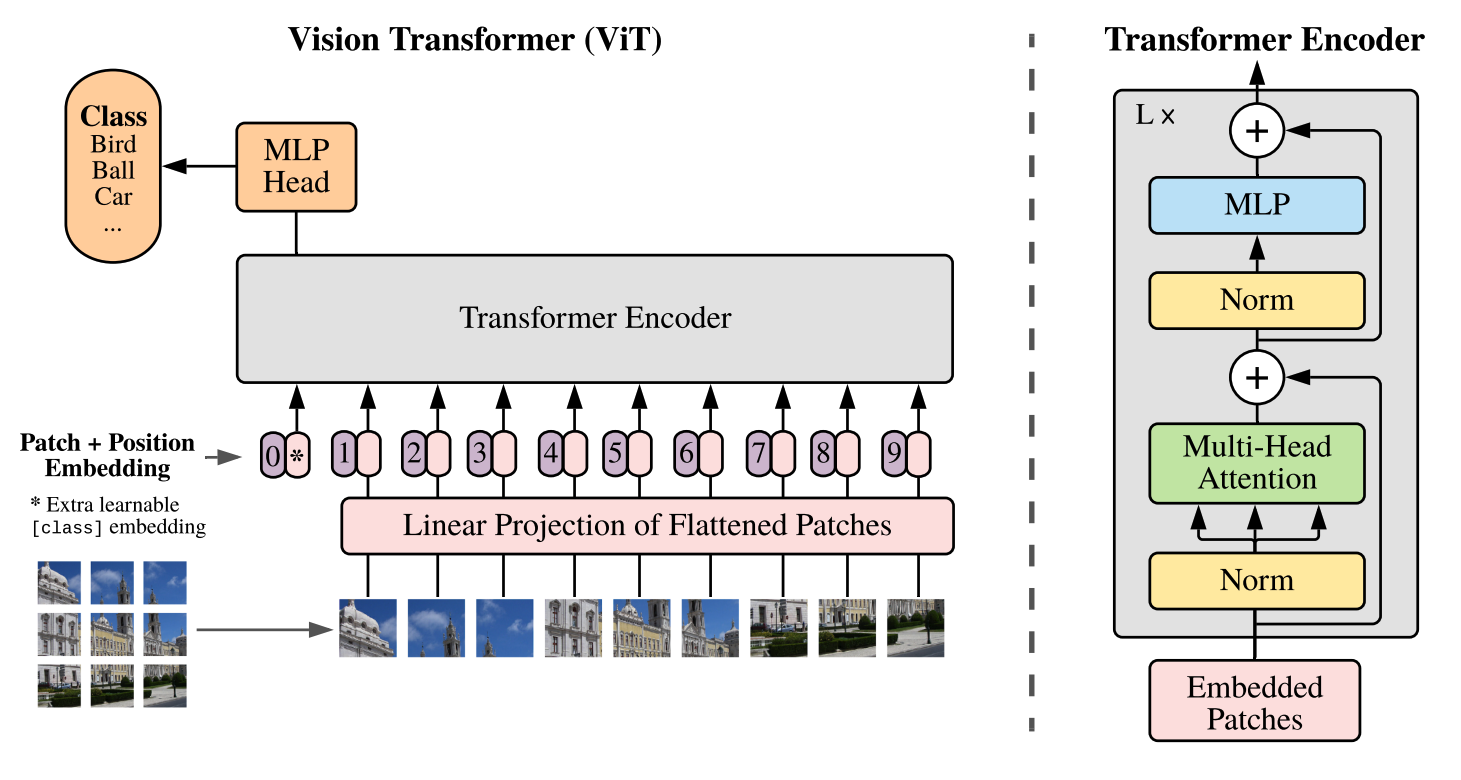
\includegraphics[width=14cm]{vit.png} \\
    \bicaption[视觉Transformer的基础框架]
      {视觉转换器的基础架构~\cite{dosovitskiy2020image}}
      {The framework of Vision Transformer}
   \label{fig:vit}
  \end{figure}

\subsubsection{视觉Transformer}
在2020年底, 完全基于自注意力机制 (Self-attention) 的视觉Transformer (Vision Transformer, ViT)的横空出世挑战了传统CNN在计算机视觉领域的绝对优势地位, 并在多个视觉任务超过ResNet等CNN模型的性能。Transformer~\cite{vaswani2017attention}最初由Google在2017年提出, 应用在自然语言处理领域(Natural Language Processing, NLP)代替传统循环神经网络(RNN)进行序列建模。这种完全基于自注意力机制的深度模型相比较于基于RNN的模型具有可并行化计算以及低内存开销的优势, 并且在一系列的机器翻译任务中取得优异的性能。Devlin 等人将 Transformer \cite{devlin2018bert} 应用至无监督NLP模型预训练任务, 并在当时11个任务上取得最先进的结果。随后, OpenAI开发了GPT-3~\cite{brown2020language}, 一个具有1750亿参数的大模型, 并且在45 TB的数据商进行预训练。模型在多个NLP的任务都取得了极佳的性能, 包括机器翻译 (Machine Translation) 、 视觉问答(Visual Question Answering, VQA)等。基于Transformer的模型展示了强大的表征能力,并且成为了NLP领域的主流模型。\par

2020年, Google的研究人员首次将基于序列建模的NLP基础模型Transformer扩展到计算机视觉任务, 设计了 Vision Transformer~\cite{dosovitskiy2020image} 。如Fig.~\ref{fig:vit}所示, Vision transformer 包含标准的 Transformer 编码器。
\begin{figure}[!htp]
    \centering
    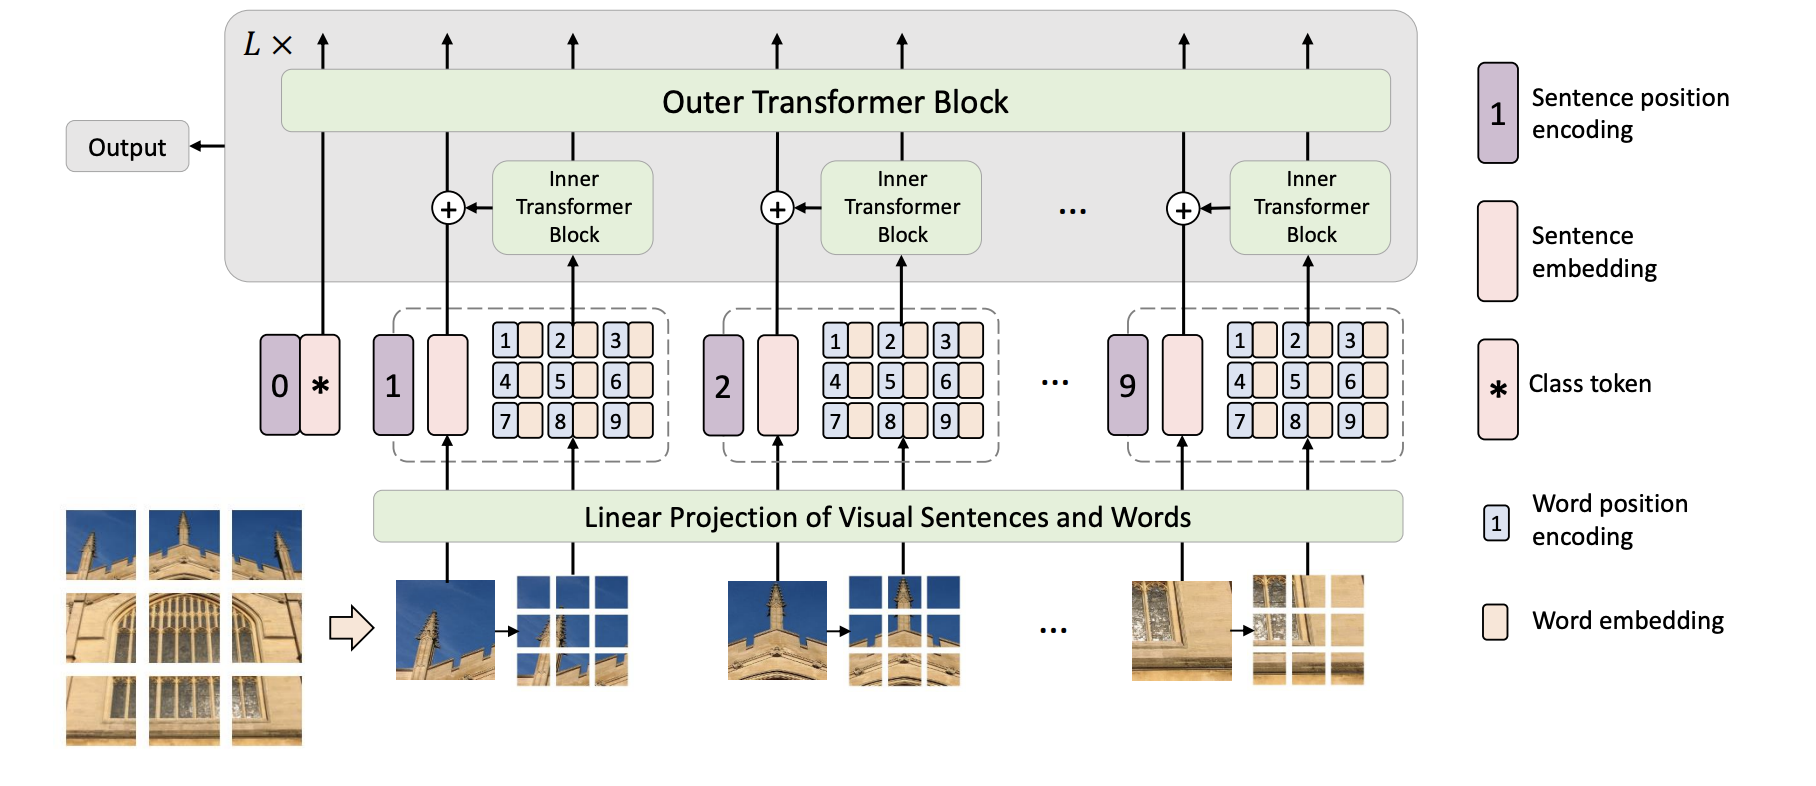
\includegraphics[width=15cm]{tit.png} \\
    \bicaption[视觉Transformer变种的基础框架, 图~\cite{han2021transformer}]
      {Transformer in Transformer 的基础架构~\cite{han2021transformer}}
      {The framework of  Transformer in Transformer}
   \label{fig:tit}
  \end{figure}

其主要模块是基于多头的注意力机制 (Multi-head Attention, MHA):
\begin{equation}
    \text { MultiHead }(Q, K, V)=\text {Concat}\left(\text {head}_1, \ldots, \text {head}_{\mathrm{h}}\right) W^O,
\end{equation}
\begin{equation}
    \text {head}_{\mathrm{i}}=\operatorname{Attention}\left(Q W_i^Q, K W_i^K, V W_i^V\right).
\end{equation}
其中 Query向量 ($Q$), Key向量 ($K$), Value向量 ($V$) 是对应序列中每一个token的三个不同的矩阵, h 是代表并行的自注意力数量, $W_i^Q$, $W_i^K$, $W_i^V$ 是对应的每一个自注意力的投射矩阵, MHA通过将多个自注意力得到的表征结果进行融合, 实现模型关注序列不同的token的效果。同时, 自注意力的表述如下:

\begin{equation}
    \operatorname{Attention}(Q, K, V)=\operatorname{softmax}\left(\frac{Q K^T}{\sqrt{d_k}}\right) V.
    \label{eq:attention}
\end{equation}
其中 $d_k$ 是 Key向量的维度。\par
为了使Transformer能处理2D的图像数据, 如\ref{fig:vit}所示, 将图片$\mathbf{x} \in \mathbb{R}^{H \times W \times C}$ 切割成一系列的图片块$\mathbf{x}_p \in \mathbb{R}^{N \times\left(P^2 \cdot C\right)}$。 其中 $H$, $W$, $C$ 是图片的高、宽、以及通道数。$N=H W / P^2$ 是得到的图片块的数量。通过对图片块进行投影降维, 可以得到类似于在自然语言处理领域的序列输入:
\begin{equation}
    \mathbf{z}_0=\left[\mathbf{x}_{\text {class }} ; \mathbf{x}_p^1 \mathbf{E} ; \mathbf{x}_p^2 \mathbf{E} ; \cdots ; \mathbf{x}_p^N \mathbf{E}\right]+\mathbf{E}_{p o s}
\end{equation}
其中 $E$是投影矩阵, 将图像块降维成低维向量, $E_{pos}$ 是图片块的位置嵌入(Position Embeddings)。由于Vision Transformer 比CNN具有更少的归纳偏置 (Inductive Bias),
\begin{figure}[!htp]
    \centering
    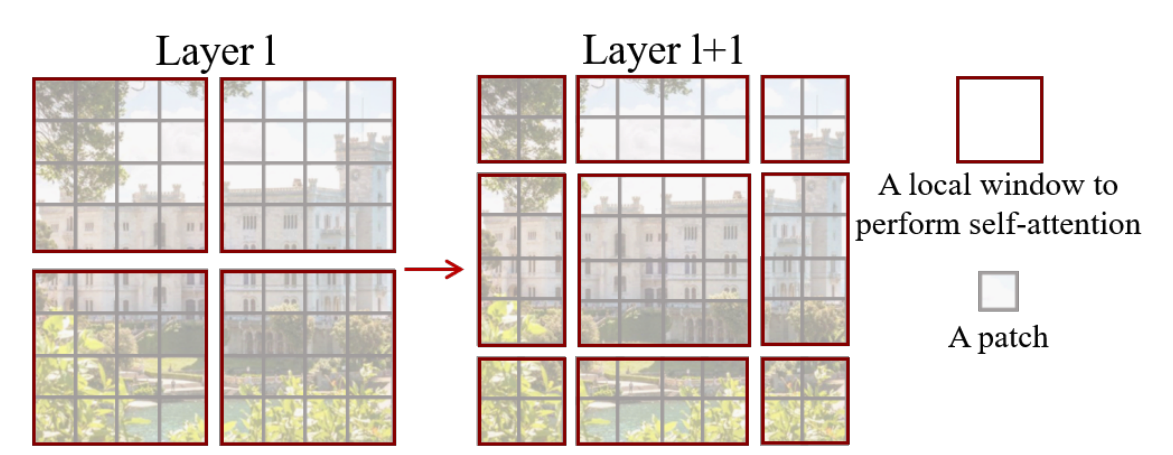
\includegraphics[width=15cm]{swin.png} \\
    \bicaption[移动窗口自注意力的计算机制, 图~\cite{liu2021swin}]
      {移动窗口自注意力的计算机制~\cite{liu2021swin}}
      {The illustration of Shifted Window Multi-head Self Attention }
   \label{fig:swin}
\end{figure}

在小规模数据集上预训练时, 没有达到CNN的性能, 然而在大规模数据集 (JFT-300M)上训练, Vision transformer 取得更优的图像分类效果。 随后, Vision transformer 开始被应用在多个计算机视觉任务, 如目标检测(Object Detection) ~\cite{carion2020end, zhu2021deformable}、语义分割 (Semantic Segmentation)~\cite{zheng2021rethinking, xie2021segformer, strudel2021segmenter, jin2021trseg, zhu2021unified}、 图像处理 (Image Processing)~\cite{chen2021pre} 等领域。 随后 Touvron等人基于原始Vision transformer提出Deit, 仅在ImageNet上进行训练, 取得 $83.1\%$的分类准确度。 在使用CNN 进行知识蒸馏 (Knowledge Distillation)后, 取得最高达 $85.2\%$的准确度。\par

2021年, 传统的Vision transformer只能刻画图片块之间的联系, 而忽略了一个图片块内部的特征。 为了解决这个问题, 如图\ref{fig:tit}, Han 等人提出一个transformer in transformer的架构, 对原始图片块继续细分成更小的图片块, 并且同时对粗粒度和细粒度的图片块进行建模。随后, CAT~\cite{lin2022cat} 和 Twins~\cite{chu2021twins} 提出交替在层间使用全局以及局部的注意力机制来减少计算复杂度以及提高表征能力。\par

由于如Eq.~\ref{eq:attention}所示, 自注意力力机制的计算复杂度随着图片块数量$N$的增长成平方增长, 使得基础的Vision transformer模型无法应用在高分辨率的视觉任务中。 2021年, ICCV的最佳论文奖得主 Swin Transformer~\cite{liu2021swin}提出在移动窗口内进行自注意力计算 (Shifted-window Self-attention), 如Fig.~\ref{fig:swin}所示, 图左是在第l层的窗口划分, 其中自注意力的计算局限于红色的窗口内。假设每一个窗口包含$M \times M$个图片块, 那么基于窗口的自注意力机制的计算复杂度 (W-MSA)可以由以下的公式表示:

\begin{figure}[!htp]
    \centering
    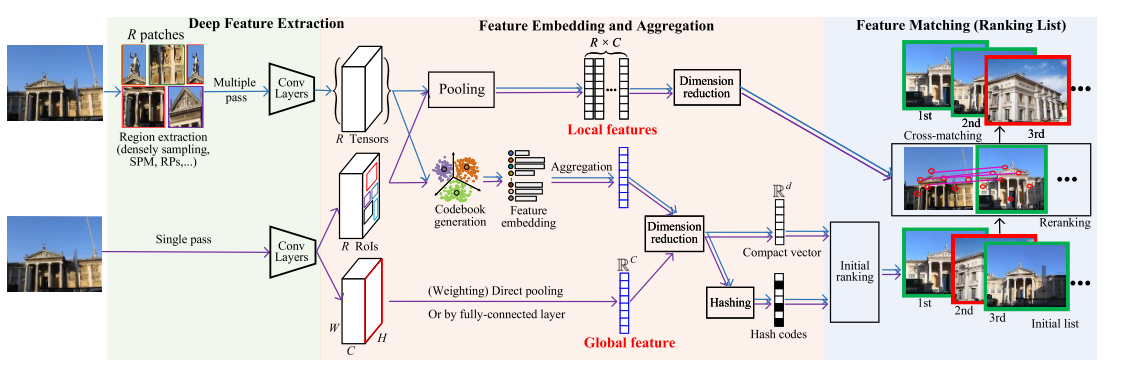
\includegraphics[width=15cm]{deepretrieval.png} \\
    \bicaption[基于预训练CNN的图像检索基本框架, 图~\cite{chen2021deep}]
      {基于预训练CNN的图像检索基本框架,从左到右, 包括图像特征提取, 特征嵌入与聚合以及最后的特征匹配阶段。~\cite{chen2021deep}}
      {The general framework of deep image retrieval based on pretrained CNN. It includes the image feature retrieval, feature embedding and aggregation and the final feature matching phases. }
   \label{fig:retrieval}
\end{figure}

\begin{equation}
    \Omega(\text { W-MSA })=4 h w C^2+2 M^2 hwC.
\end{equation}

其中$hw$是图片块的数量。由此可知, Swin-transformer 的计算复杂度随着图像大小可以呈线性增长, 具有可扩展性。Swin Transformer在图像分类, 目标检测等领域都达到了最先进的性能, 开始成为计算机视觉领域的主干模型~\cite{tianyonglin22,xsx2022,cyf2023,sxf2023,yuhang2021,  jfh2021, wfp2022,  liu2021swinnet,liu2022video, huang2022swin, cao2021swin, ma2022swinfusion}。在本文中, 我们第一个探索Vision transformer在大规模图像检索领域的应用, 并且取得了优异的性能。

\subsection{基于深度特征的图像检索}
在深度学习时代的图像检索方法主要分为两种: (1) 基于预训练CNN的特征提取 (2)基于任务的微调。早期的基于深度学习的检索方法基于两阶段检索, 即使用在图像分类数据集如ImageNet进行分类任务训练后的CNN代替基于人工的特征提取方法,如SIFT, 进行特征提取, 第二阶段如Sec.~\ref{sec:manual}, 使用 VLAD、 BoW 或者 FV 生成全局的表征向量。 而基于端到端的检索, 则使用图像的监督标签, 端到端训练的生成用于图像检索的表征向量, CNN 会在监督训练的过程中调整学习适用于特定任务的图像特征。

\subsubsection{基于预训练CNN的特征提取}
一部分基于预训练CNN提取特征的工作一般也包含两个阶段: ``特征提取'' 与 ``特征聚合''。``\textbf{特征提取}'': 如图所示, 一部分工作从全连接层得到特征向量
\begin{figure}[!htp]
    \centering
    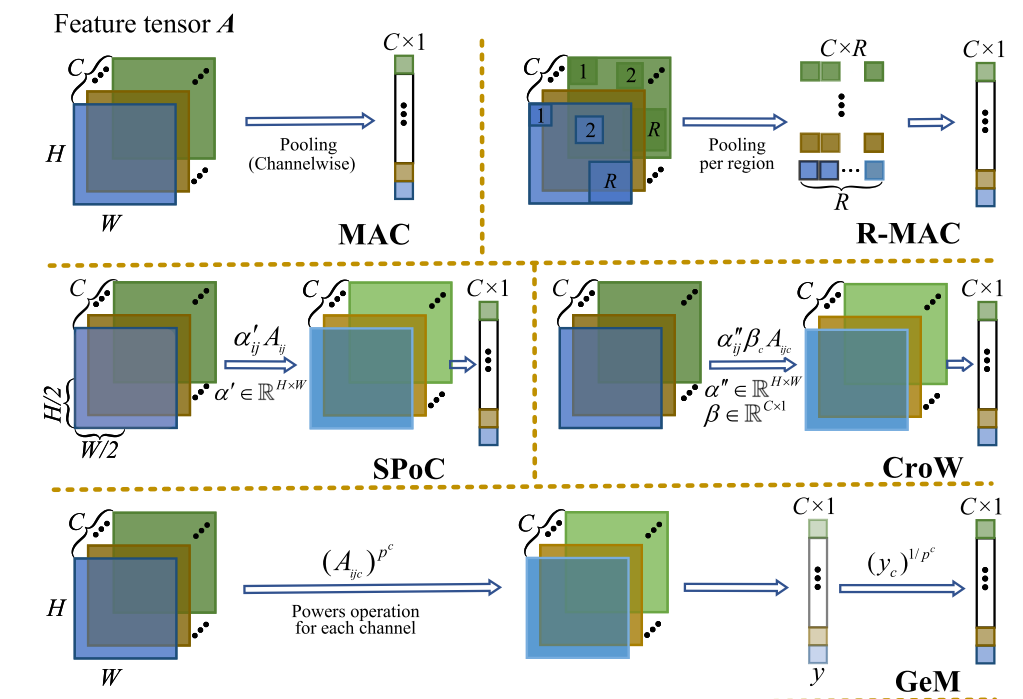
\includegraphics[width=15cm]{feature_agg.png} \\
    \bicaption[特征聚合的几种常用的方法]
      {特征聚合的几种经典的算法.}
      {The illustration of canonical feature aggregation algorithms.}
   \label{fig:featureagg}
\end{figure}
, 类似手工特征提取方案的全局特征描述符,然后使用PCA 降维以及标准化~\cite{sharif2014cnn,gong2014multi}。然而, 基于全连接层的特征向量损失了图像的空间信息, 缺乏局部几何不变性~\cite{gong2014multi}。因此, 另一部分研究人员研究使用卷积层后的特征图进行图像检索。2016年, Razavian~\cite{razavian2016visual} 提取CNN最后一个卷积层的多尺度特征, 并且通过空间池化(Spatial Pooling) 降维用于检索。随后 Morere 提出嵌套不变池化 (Nested Invariance Pooling )来生成用于检索的全局描述符~\cite{morere2017nested}。在2017年 Albert \cite{jimenez2017class} 等人提出 Class Activation Maps (CAM) 来对CNN的卷积特征图生成每个类别不同的权重图。随后这些权重图经过池化得到对应的类向量。最后的全局特征向量是所有类向量经过PCA降维以及标准化后的集成。2018年, Yihang~\cite{lou2018multi} 提出 MSCAN, 一个多尺度的注意力网络来生成全局特征描述符。通过使用 Long Short-Term Memory (LSTM) 网络来对不同卷积层后的特征图建模, 以及使用注意力机制对每一层的特征图加权, 模型可以学习到不同尺度的注意力, 从而提高检索的性能。\par
``\textbf{特征聚合}'': 将CNN得到的卷积特征图聚合成适用于检索任务的紧凑的全局特征向量。一种最简单的方式是通过最大池化 (Max Pooling) 、平均池化(Average Pooling) 等~\cite{razavian2016visual, pang2018unifying}。
2016年, Razavian 提出MAC~\cite{razavian2016visual} 如Fig.~\ref{fig:featureagg}所示, 在通道域进行最大池化操作, 如Eq.~\ref{eq:mac}。
\begin{equation}
    \mathbf{f}^{(m)}=\left[\mathrm{f}_1^{(m)} \ldots \mathrm{f}_k^{(m)} \ldots \mathrm{f}_K^{(m)}\right]^{\top}, \quad \mathbf{f}_k^{(m)}=\max _{x \in \mathcal{X}_k} x.
    \label{eq:mac}
\end{equation}
其中 $\mathcal{X}$是卷积生成的特征图, $k$ 是对应的特征图的通道。
Tolias 等人提出R-MAC~\cite{tolias2015particular}在特征图中分块进行最大池化, 然后再聚合成一个全局特征向量,这样可以保留更多的局部信息,便于检索。Babenko 提出 SPoC~\cite{babenko2015aggregating} 如图 Fig.~\ref{fig:featureagg}, 作者先使用Gaussian weighting对特征图进行加权:
\begin{equation}
    \alpha_{(x, y)}=\exp \left\{-\frac{\left(y-\frac{H}{2}\right)^2+\left(x-\frac{W}{2}\right)^2}{2 \sigma^2}\right\}
    \label{eq:gaussianweight}
\end{equation}
其中$x$, $y$是在特征图中的坐标, $H$, $W$是特征图的长和宽。 加权之后的特征图经过求和池化 (Sum Pooling)后得到全局特征向量如下。
\begin{equation}
    \mathbf{f}^{(a)}=\left[\mathrm{f}_1^{(a)} \ldots \mathrm{f}_k^{(a)} \ldots \mathrm{f}_K^{(a)}\right]^{\top}, \quad \mathrm{f}_k^{(a)}= \sum_{x \in \mathcal{X}_k} x
\end{equation}
2017年 Radenovi´ 提出 GeM~\cite{radenovic2018fine} 基于广义平均 (Generalized Mean)进行池化操作。
\begin{equation}
    \mathbf{f}^{(g)}=\left[\mathbf{f}_1^{(g)} \ldots \mathbf{f}_k^{(g)} \ldots \mathbf{f}_K^{(g)}\right]^{\top}, \quad \mathbf{f}_k^{(g)}=\left(\frac{1}{\left|\mathcal{X}_k\right|} \sum_{x \in \mathcal{X}_k} x^{p_k}\right)^{\frac{1}{p_k}}
\end{equation}
其中$p_k$ 可以视为一个超参进行手动设置, 也可以通过反向传播进行梯度训练。\par
除了通过各种池化操作从卷积特征图生成全局特征向量, 另一部分的工作通过将特征图视为多个局部特征向量的组合, 通过特征编码的方式聚合成一个全局向量。常见的有基于BoW ~\cite{li2016exploiting, mohedano2016bags, zheng2016accurate}特征编码的检索工作, 基于 VLAD~\cite{gong2014multi, yue2015exploiting}的工作以及基于FV~\cite{jegou2011aggregating, sanchez2013image}的工作。 

\subsubsection{基于任务的微调}
基于预训练CNN特征提取然后进行检索的方法有一个较大的缺陷。基于ImageNet的图像分类任务进行预训练的模型应用在其他的视觉任务, 由于与训练的图像数据和检索任务的图像数据有较大的差异 (Domain Gap), 预训练好的CNN难以在当前任务的图像数据提取出准确的图像特征, 从而无法应用于精确的检索任务中。基于任务的微调方法, 一般通过使用不同的神经网络架构, 采取不同的采样策略, 以及设计不同的损失函数来监督更新CNN的参数。
\begin{figure}[!htp]
    \centering
    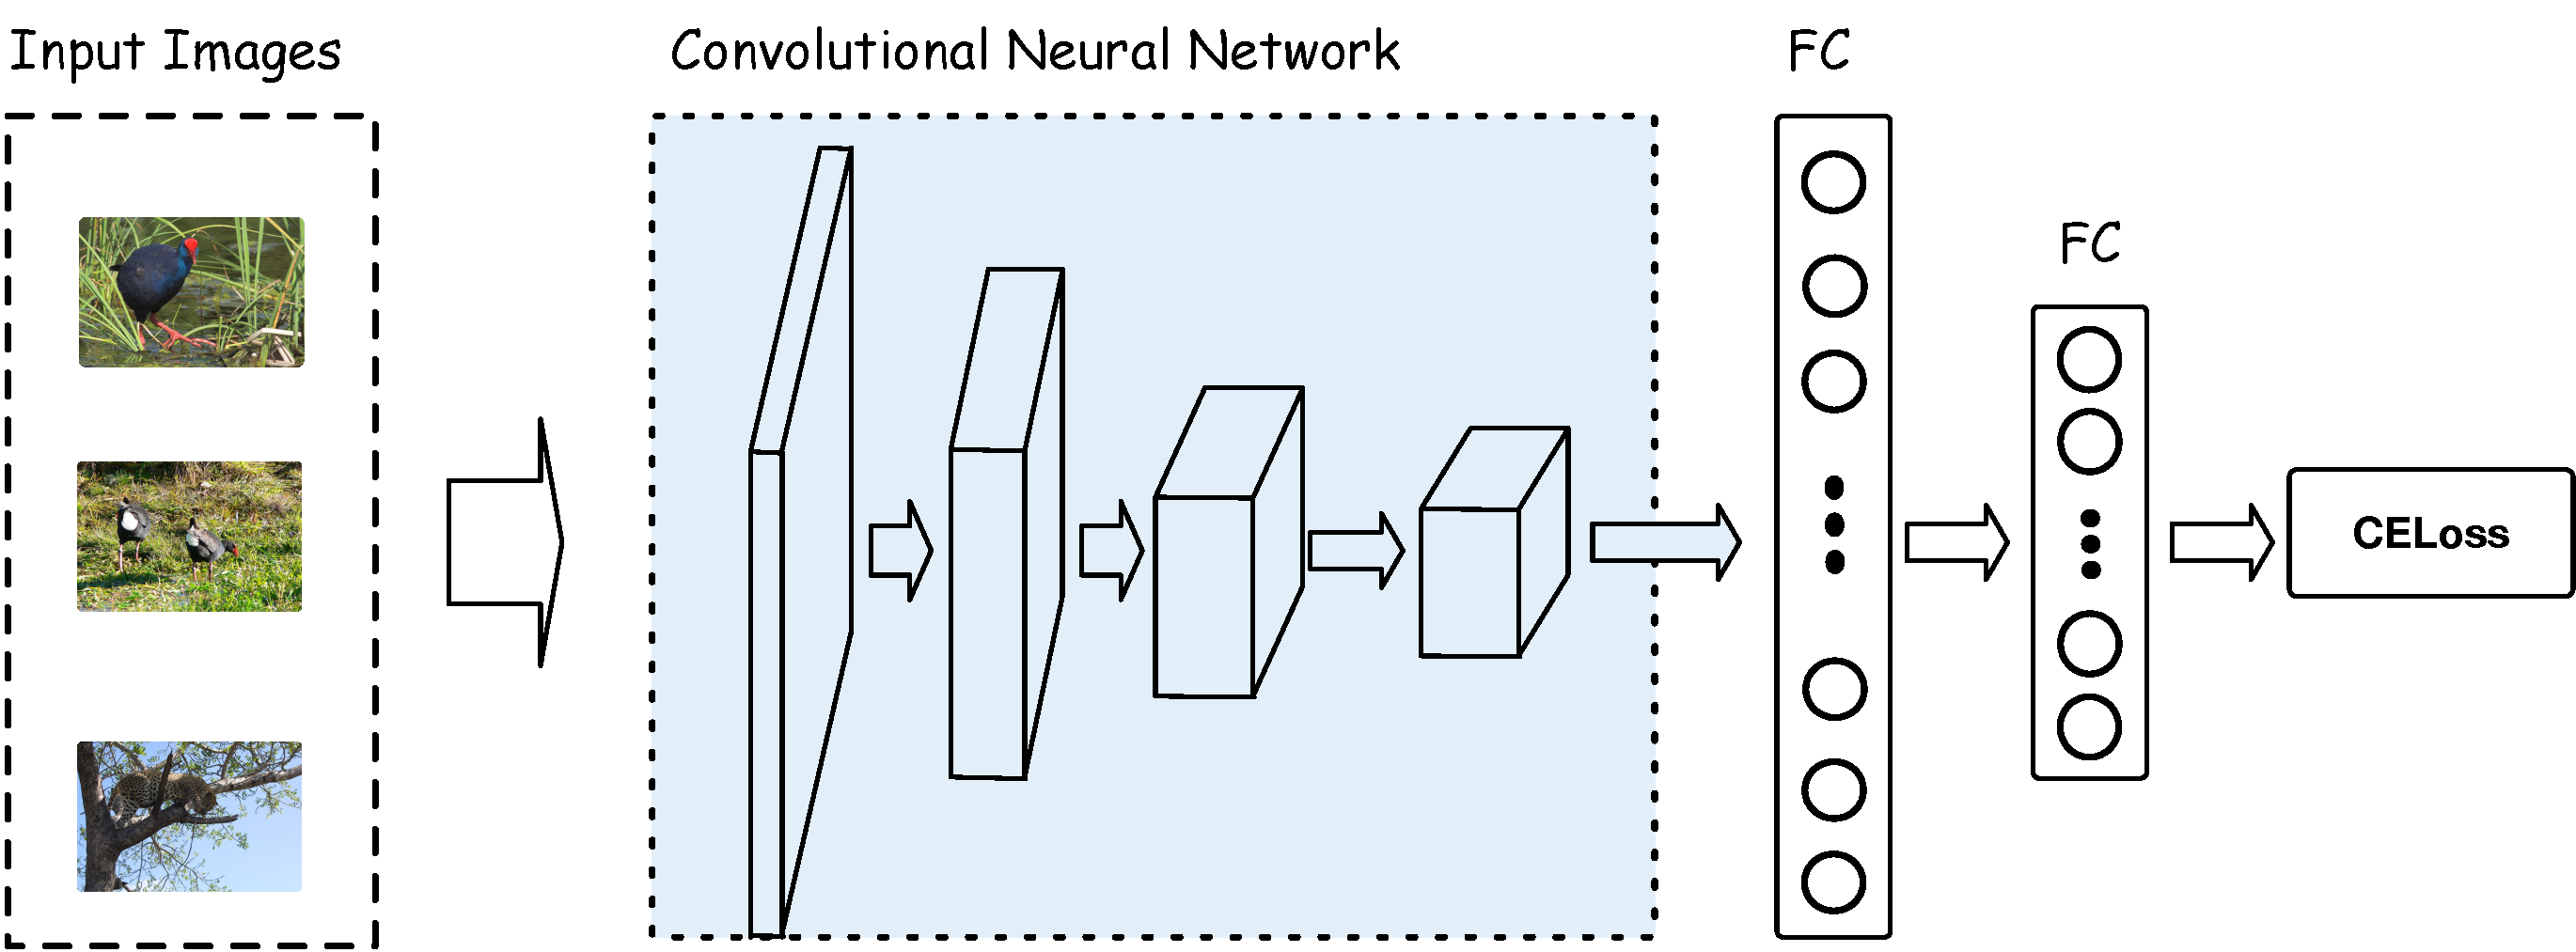
\includegraphics[width=15cm]{singlestream.pdf} \\
    \bicaption[基于分类损失函数的图像检索架构]
      {基与分类损失的CNN架构微调架构。从左至右是输入的图片, 提取特征的主干CNN网络, 以及全连接层和交叉熵损失函数}
      {The framework of convolutional Neural Network based image retrieval with categorial loss. The input images are on the left. The middle is the convolutional neural network backbone. Meanwhile, an additional fully connected layer is appended for the classification loss.  }
   \label{fig:featurestream}
\end{figure}

一般基于任务的微调方法也分为基于监督标签的监督训练微调(Supervised Fine-tuning) 以及无监督训练微调 (Unsupervised Finetuning)的方法。本文主要介绍基于监督训练的微调方法的主要架构以及发展。\par
\textbf{基于分类损失的微调方法:} 基于分类损失函数的微调方法, 根据图像检索数据集提供的标签, 在基础的主干神经网络例如AlexNet、VGG、 GoogleNet后添加一个全连接层用于分类, 然后使用交叉熵 (Cross Entropy)损失函数以及随机梯度下降进行端到端的训练优化CNN的参数。 基本的神经网络架构如图Fig.~\ref{fig:featurestream} 所示。一般做法需要在基础的架构后添加一个全连接层, 全连接层的输出维度是图片的类的数量。 对于单分类的数据集, 标准的基于交叉熵的损失函数如下:
\begin{equation}
    \mathcal{L}_{C E}\left(\hat{p}_i, y_i\right)=-\sum_i^c\left(y_i \times \log \left(\hat{p}_i\right)\right).
\end{equation}
其中 $y_i$ 是真实的标签, $\hat{p}_i$ 是模型输出的概率。$c$是总共的类的数量。而对于一张图片可能具有多个标签的检索数据集, 一般使用sigmoid函数激活, 交叉熵损失函数如下所示:
\begin{equation}
    \text { Loss }=-\sum_{i=1}^c(y \log (\hat{p})+(1-y) \log (1-\hat{p}))
    \label{eq:ce}
\end{equation} \par
2014年, Babenko~\cite{babenko2014neural} 提出第一个基于AlexNet微调的图像检索框架, 通过实验证实在图像数据集上进行重新的分类训练可以提高模型的检索性能。 \par

\begin{figure}[!htp]
    \centering
    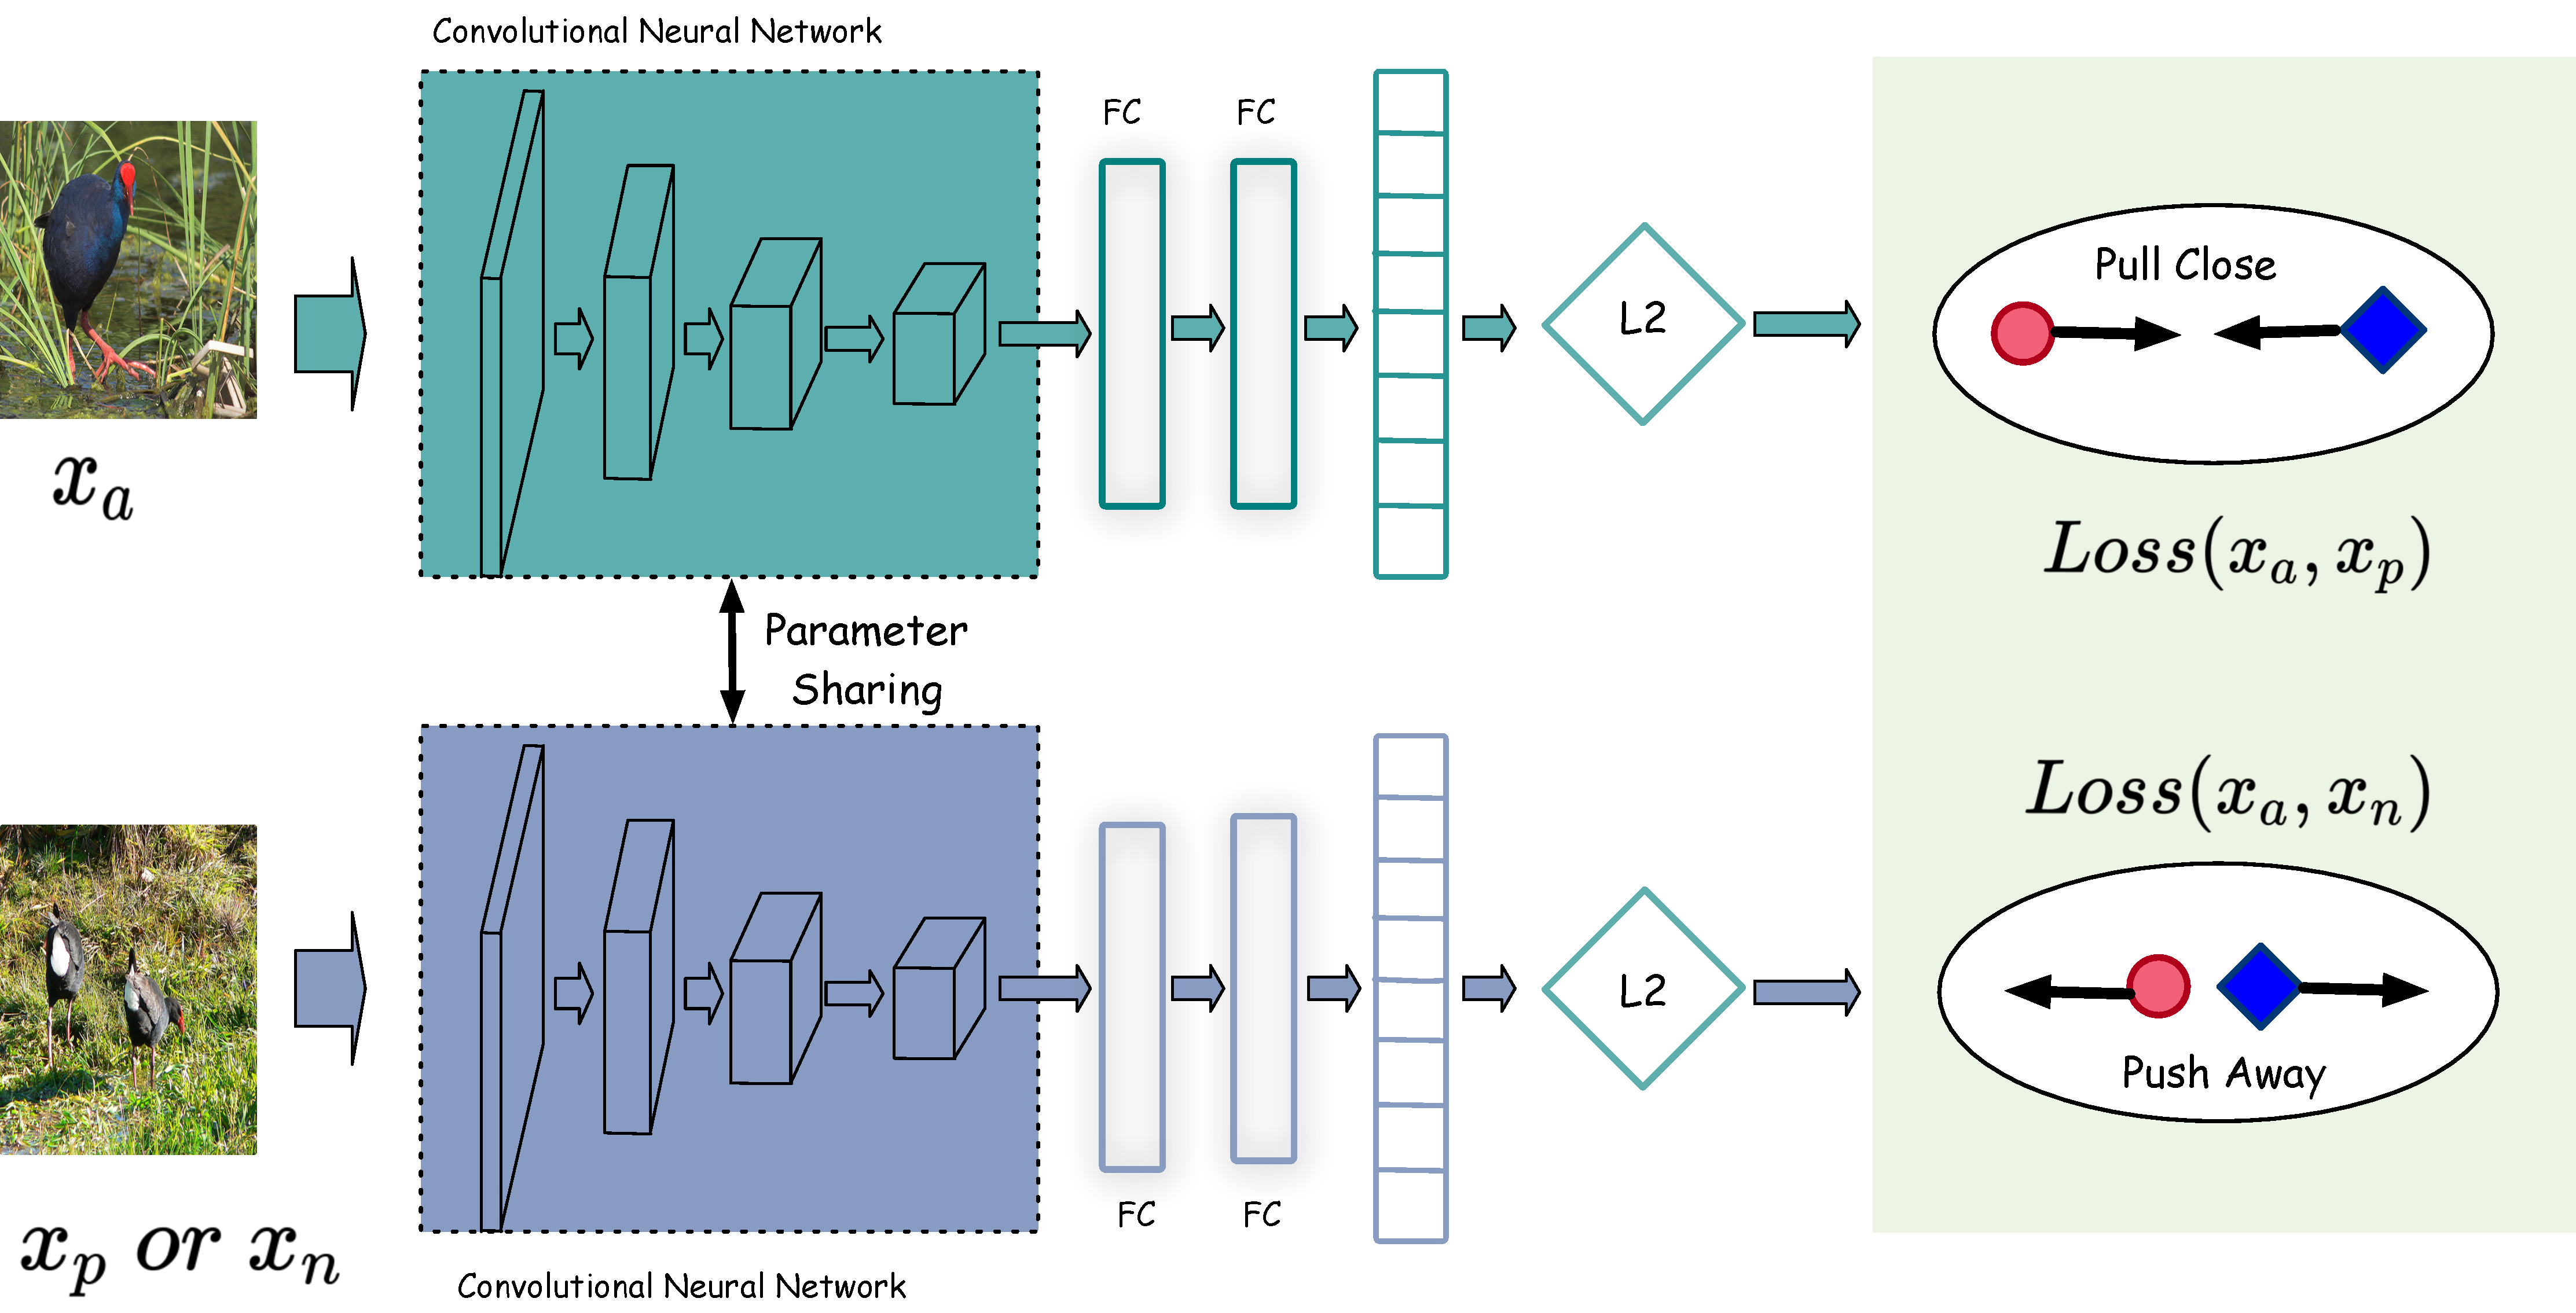
\includegraphics[width=15cm]{siamese.pdf} \\
    \bicaption[基于孪生神经网络的图像检索架构]
      {基与孪生CNN架构的微调图像检索架构。输入的图片以图片对的形式同时输入权重共享的CNN中, 使用对比损失来拉近相同标签图片的表征, 拉远不同标签的表征}
      {The framework of siamese convolutional Neural Network based image retrieval with contrastive loss. The input images are organized in pairs. The pairwise contrastive loss is adopted to push away representations from negative image pairs and pull close those from positive pairs }
   \label{fig:siamese}
\end{figure}

2017年, Noh~\cite{noh2017large}引入注意力机制并且通过监督训练同步学习注意力网络以及CNN的参数, 让卷积神经网络可以学习到局部的细粒度特征。 \par
2020年, Cao~\cite{cao2020unifying} 提出在模型中同时集成全局和局部的特征。作者使用GeM 池化来得到全局向量, 同时使用ArcFace~\cite{deng2019arcface} 损失函数, 使得类内的向量尽量近, 类间的
向量距离尽量远。对于局部特征的学习, 使用自编码器 (Auto Encoder)缩小卷积特征图的尺度, 并且使用注意力机制以及基于softmax的分类损失函数进行端到端的监督训练。 \par
\textbf{基于孪生神经网络的微调方法:} 孪生卷积神经网络是两个完全一致的CNN共享所有的参数。孪生神经网络的输入是图片对 $(x_i, x_j)$, 监督信号是 0 或者 1, 如果两张图片是标签一致, 则 $\mathcal{S}(x_i, x_j) = 1$, 如果两张图片标签不一致, 则 $\mathcal{S}(x_i, x_j) = 0$。 通用的成对对比损失函数如下 (Pairwise Contrastive Loss):
\begin{equation}
    \begin{aligned}
        \mathcal{L}_{\text {PCS }}\left(x_i, x_j\right) & =\frac{1}{2} \mathcal{S}\left(x_i, x_j\right) \mathcal{D}\left(x_i, x_j\right)+ \\
        & \frac{1}{2}\left(1-\mathcal{S}\left(x_i, x_j\right)\right) \max \left(0, m-\mathcal{D}\left(x_i, x_j\right)\right)
        \end{aligned}.
        \label{eq:siamese}
\end{equation}
其中$m$ 是一个需要设定的间距参数, $\mathcal{D}$ 是一个距离函数, 通常情况下是用欧式距离代替。在Eq.~\ref{eq:siamese}中可以看到如果图片对不属于同一类别即$\mathcal{S}(x_i, x_j) = 0$ 不属于同一类别, 则 
\begin{figure}[!htp]
    \centering
    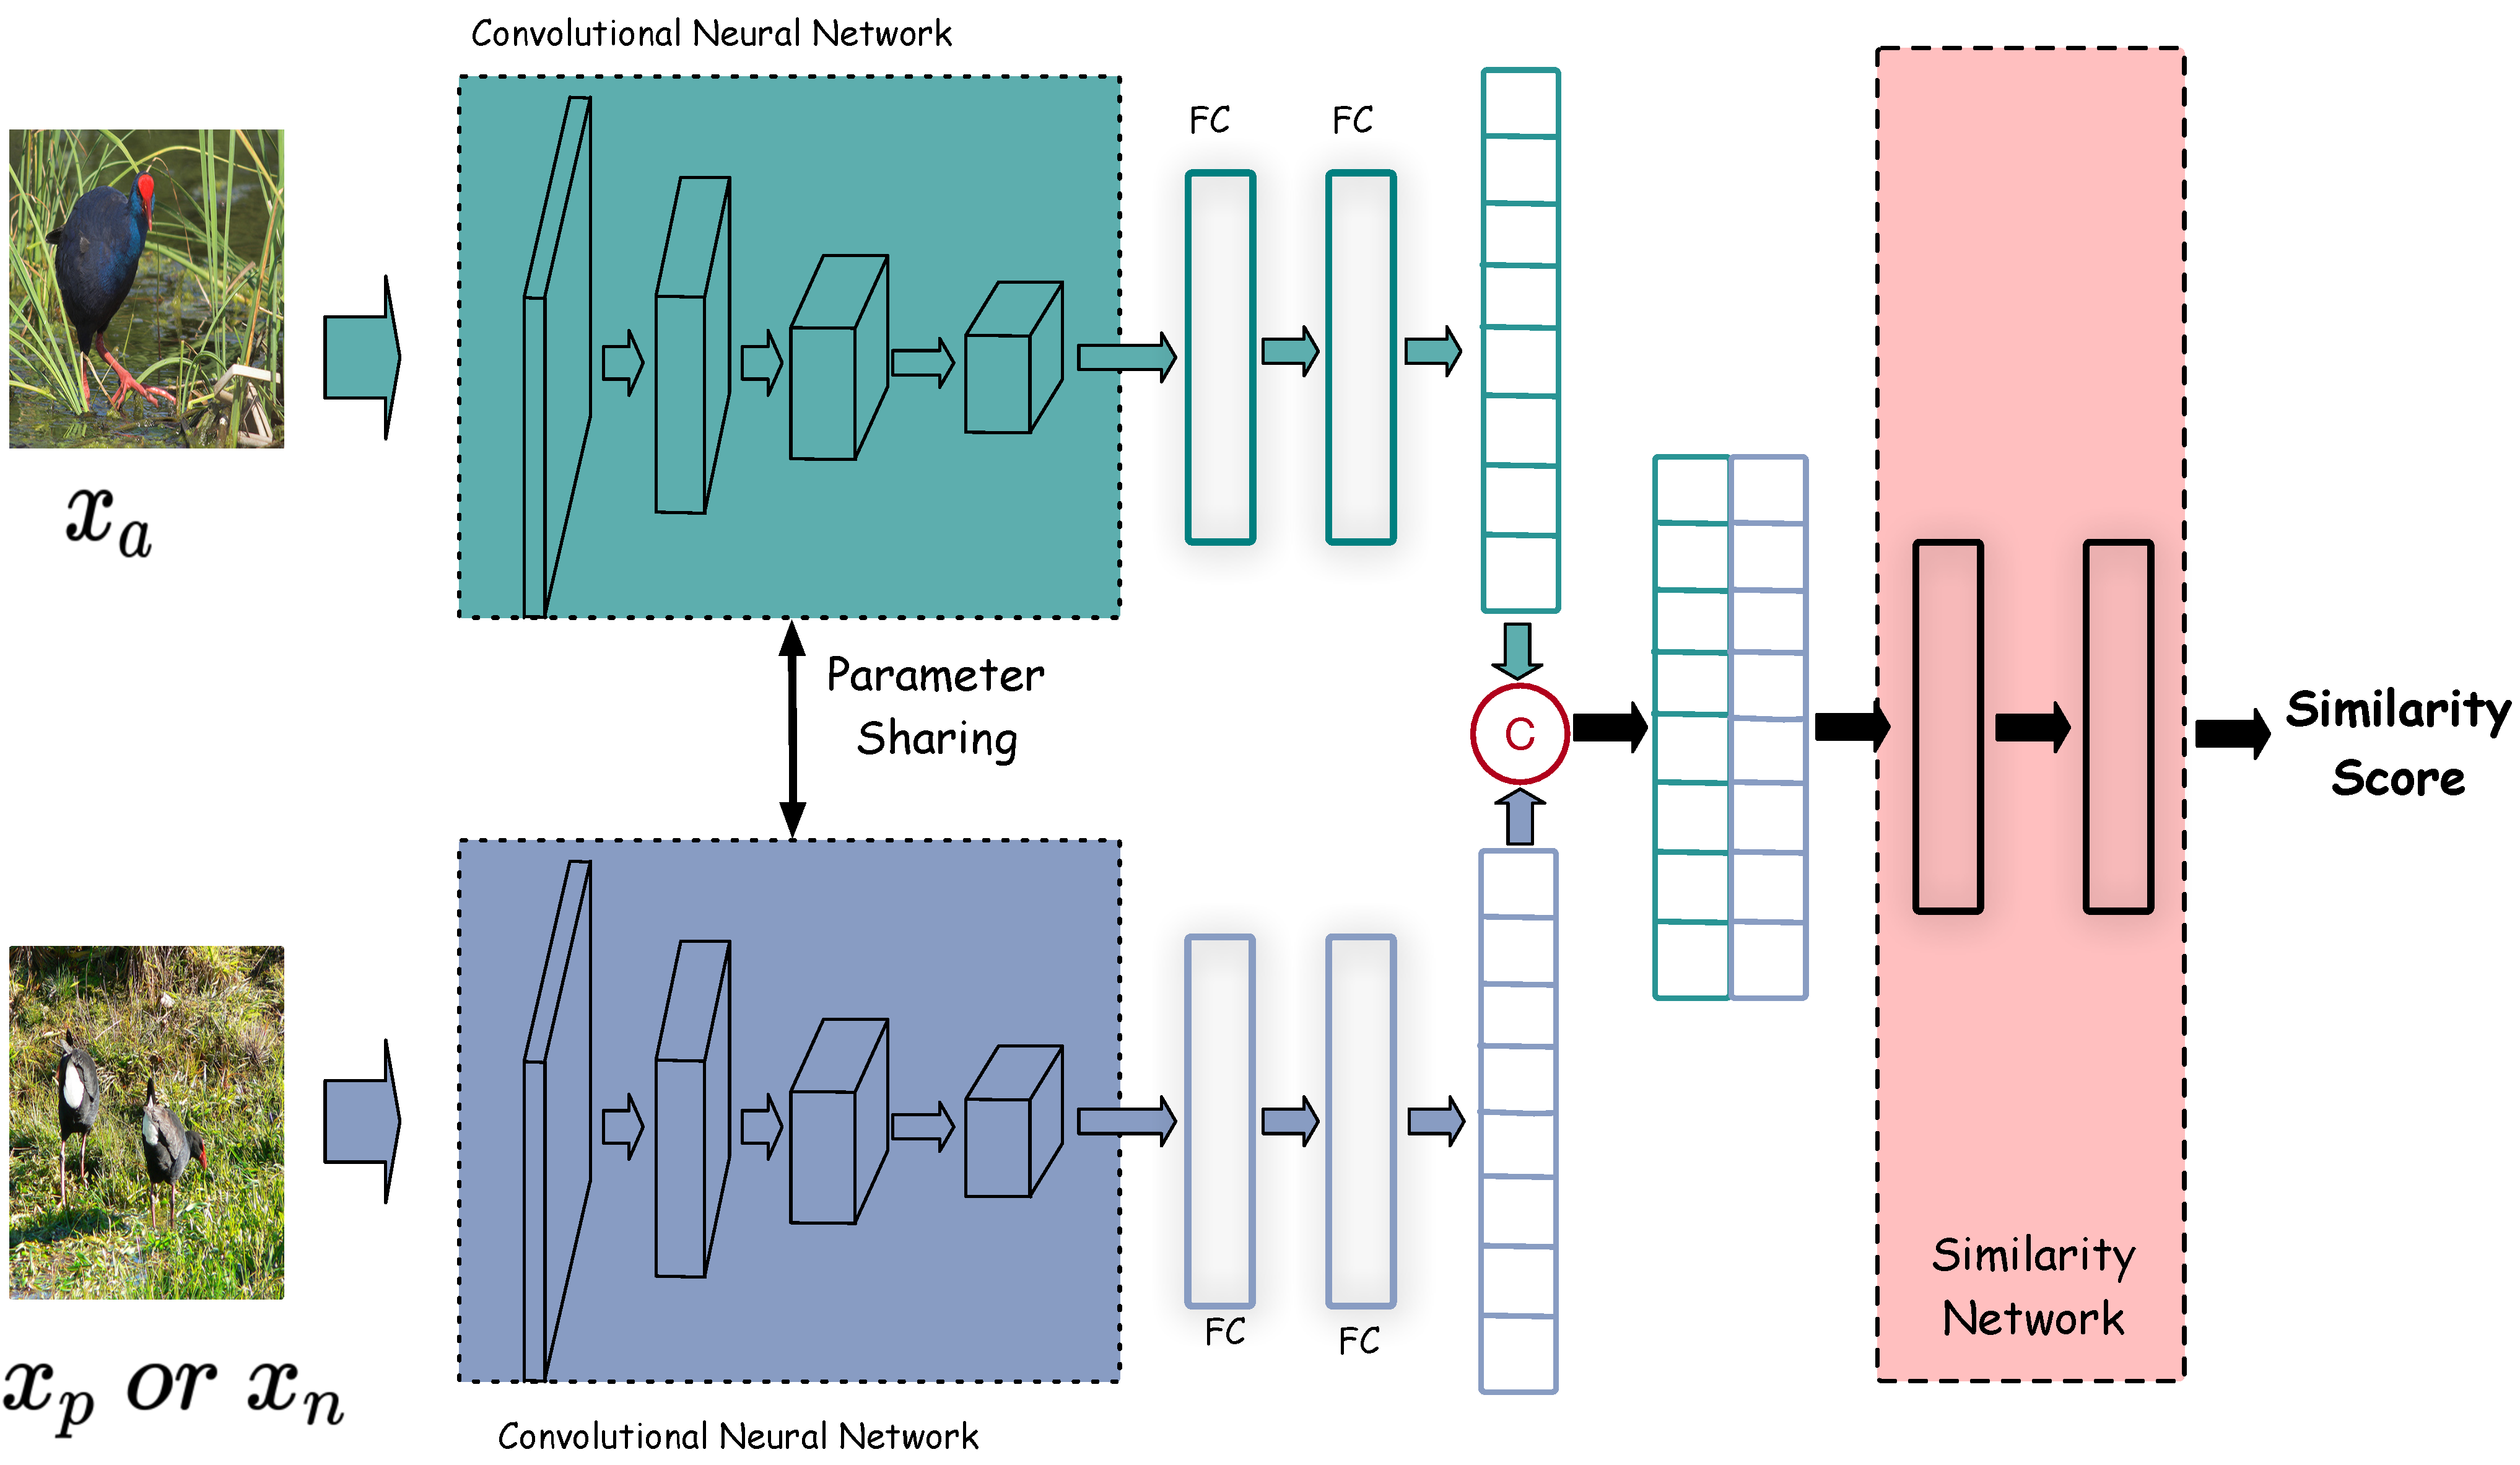
\includegraphics[width=15cm]{siamese_variant.pdf} \\
    \bicaption[基于孪生神经网络的第二种图像检索架构]
      {基于孪生CNN架构的微调的另一种架构, 通过在拼接两个卷积神经网络的输出, 然后使用一个计算相似度的全连接网络生成相似度的评分。}
      {The framework of another siamese convolutional neural network based image retrieval. It concatenate the output from two indential convolutional backbones and output a similarity score by using a fully-connected similarity network.}
   \label{fig:siamesevariant}
\end{figure}


$\mathcal{D}(x_i,x_j)$ 需要大到接近 $m$ 才能使损失最小。反而, 如果属于同一类别, 则损失函数使得图片对的表征距离 $\mathcal{D}(x_i, x_j)$ 尽量接近 0。\par
2016年, Li~\cite{li2015feature} 等人提出基于孪生神经网络进行端到端的训练用于图像检索。作者使用基于最大似然估计来优化参数, 本质上是使用sigmoid 交叉熵损失函数进行图片对的二分类, 并且取得了优异的检索性能。 \par
2017年, Eng-Jon~\cite{Eng-Jon} 基于孪生卷积神经网络, 在卷积特征图后使用Fisher Vector算法来代替传统的池化方法提取全局特征向量, 然后基于对比损失函数进行神经网络优化训练。\par
2018年, Radenovi ~\cite{radenovic2018fine} 则基于 GeM 池化算法得到全局的特征向量, 同时使用对比损失进行成对的监督学习。 \par
尽管基于孪生网络对比损失的微调图像检索方法在精度上优于基于分类损失的算法, 孪生对比损失函数有一个明显的缺陷, 由Eq.~\ref{eq:siamese} 可知, 对于相似的图片对, 此损失函数会将损失降低到无限趋近于0, 也就是两个向量需要完全一致。由于图片内容的迥异, 正样本对的特征可能会有差距, 直接映射到相同的一点会造成神经网络学习困难, 导致性能的下降。 \par
Cao ~\cite{cao2016quartet} 提出Quartet-net 使用双间隔对比损失函数(Double Margin Contrastive Loss)来监督训练:
\begin{equation}
    \begin{array}{r}
        \mathcal{L}_{\mathcal{D}_{-} S i a m}\left(x_i, x_j\right)=\frac{1}{2} \mathcal{S}\left(x_i, x_j\right) \max \left(0, \mathcal{D}\left(x_i, x_j\right)-m_1\right)+ \\
        \frac{1}{2}\left(1-\mathcal{S}\left(x_i, x_j\right)\right) \max \left(0, m_2-\mathcal{D}\left(x_i, x_j\right)\right).
        \end{array}
        \label{eq:doublem}
\end{equation}
其中$m_1 > 0$ 并且 $m_2 > 0$ 是对应对于正样本对和负样本对的间隔参数。由 Eq.~\ref{eq:doublem}所知, 对于正样本对, 也就是 $\mathcal{S}_{x_i, x_j} = 1$, 损失函数只会使两个向量的距离接近$m_1$ 而不是接近 $0$。同时, 文章使用一个模仿学习 (Mimic Learning), 额外引入一个教师卷积神经网络 (Teacher CNN ),模仿学习的损失函数如下:
\begin{equation}
    E(\mathbf{x})=\frac{1}{2}\left\|\mathbf{z}_S-\mathbf{z}_T\right\|_2^2.
\end{equation}
$\mathbf{z}_S$ 和 $\mathbf{z}_{T}$ 是教师CNN和学生CNN的概率输出。其中学生CNN是由Eq.~\ref{eq:doublem}进行训练, 通过引入模仿学习, 可以防止学生CNN过拟合。 \par
另一种基于孪生神经网络的检索架构不基于对比损失函数,  基本的框架如图所示Fig.~\ref{fig:siamesevariant}。通过将两个分支的特征向量拼接, 新增一个基于全连接的神经网络输出这个拼接向量的相似度。 典型的应用有:\par
2016年, Lin 提出 PersonNet~\cite{wu2016personnet} 是基于VGG设计的孪生神经网络。与Fig.~\ref{fig:siamesevariant}不同在于, PersonNet 在两个卷积层后拼接, 然后通过卷积网络最后生成相似度分数。 \par
随后, 2017年, zhedong等人~\cite{zheng2017discriminatively} 基于此架构设计一个用于行人检索的孪生网络架构。不同点在于,模型最后生成的是一个2维向量, 即图片对属于同一类以及不同类的概率。随后使用交叉熵损失函数来监督。 同时, 作者在每一个分支后面添加了分类损失函数, 使得模型在学会分辩图片对的相似度的同时可以保留对每个人的辨识度。
\subsubsection{基于三元神经网络的检索方法}
三元卷积神经网络是由三个完全一致的CNN共享所有的参数组成。模型的输入是一个三元图片组 $(x_a, x_p, x_n)$, 其中 $x_a$ 叫做基准图片(Anchor Image), $x_p$ 叫做正样本图片 (Positve Image)是和 $x_a$ 标签一致的的图片, $x_n$ 叫做负样本图片 (Negative Image)是和 Anchor 标签不一致的图片。 经典的适用于三元神经网络的损失函数(Triplet Loss)如下:
\begin{equation}
    \mathcal{L}_{\text {Triplet }}\left(x_a, x_p, x_n\right)=\max \left(0, m+\mathcal{D}\left(x_a, x_p\right)-\mathcal{D}\left(x_a, x_n\right)\right).
    \label{eq:triplet}
\end{equation}
$m$ 是间隔参数, 一般由手动设定。
$
    \rho\left(x_i, x_j\right)=\left\|f\left(x_i ; \boldsymbol{\theta}\right)-f\left(x_j ; \boldsymbol{\theta}\right)\right\|_2^2
$ 是欧式距离。 由公式可知, 损失函数会尽量拉进正样本对的距离,并且使其到负样本的距离间隔比到正样本距离间隔超过 $m$, 从而使得损失最低。 \par

\begin{figure}[!htp]
    \centering
    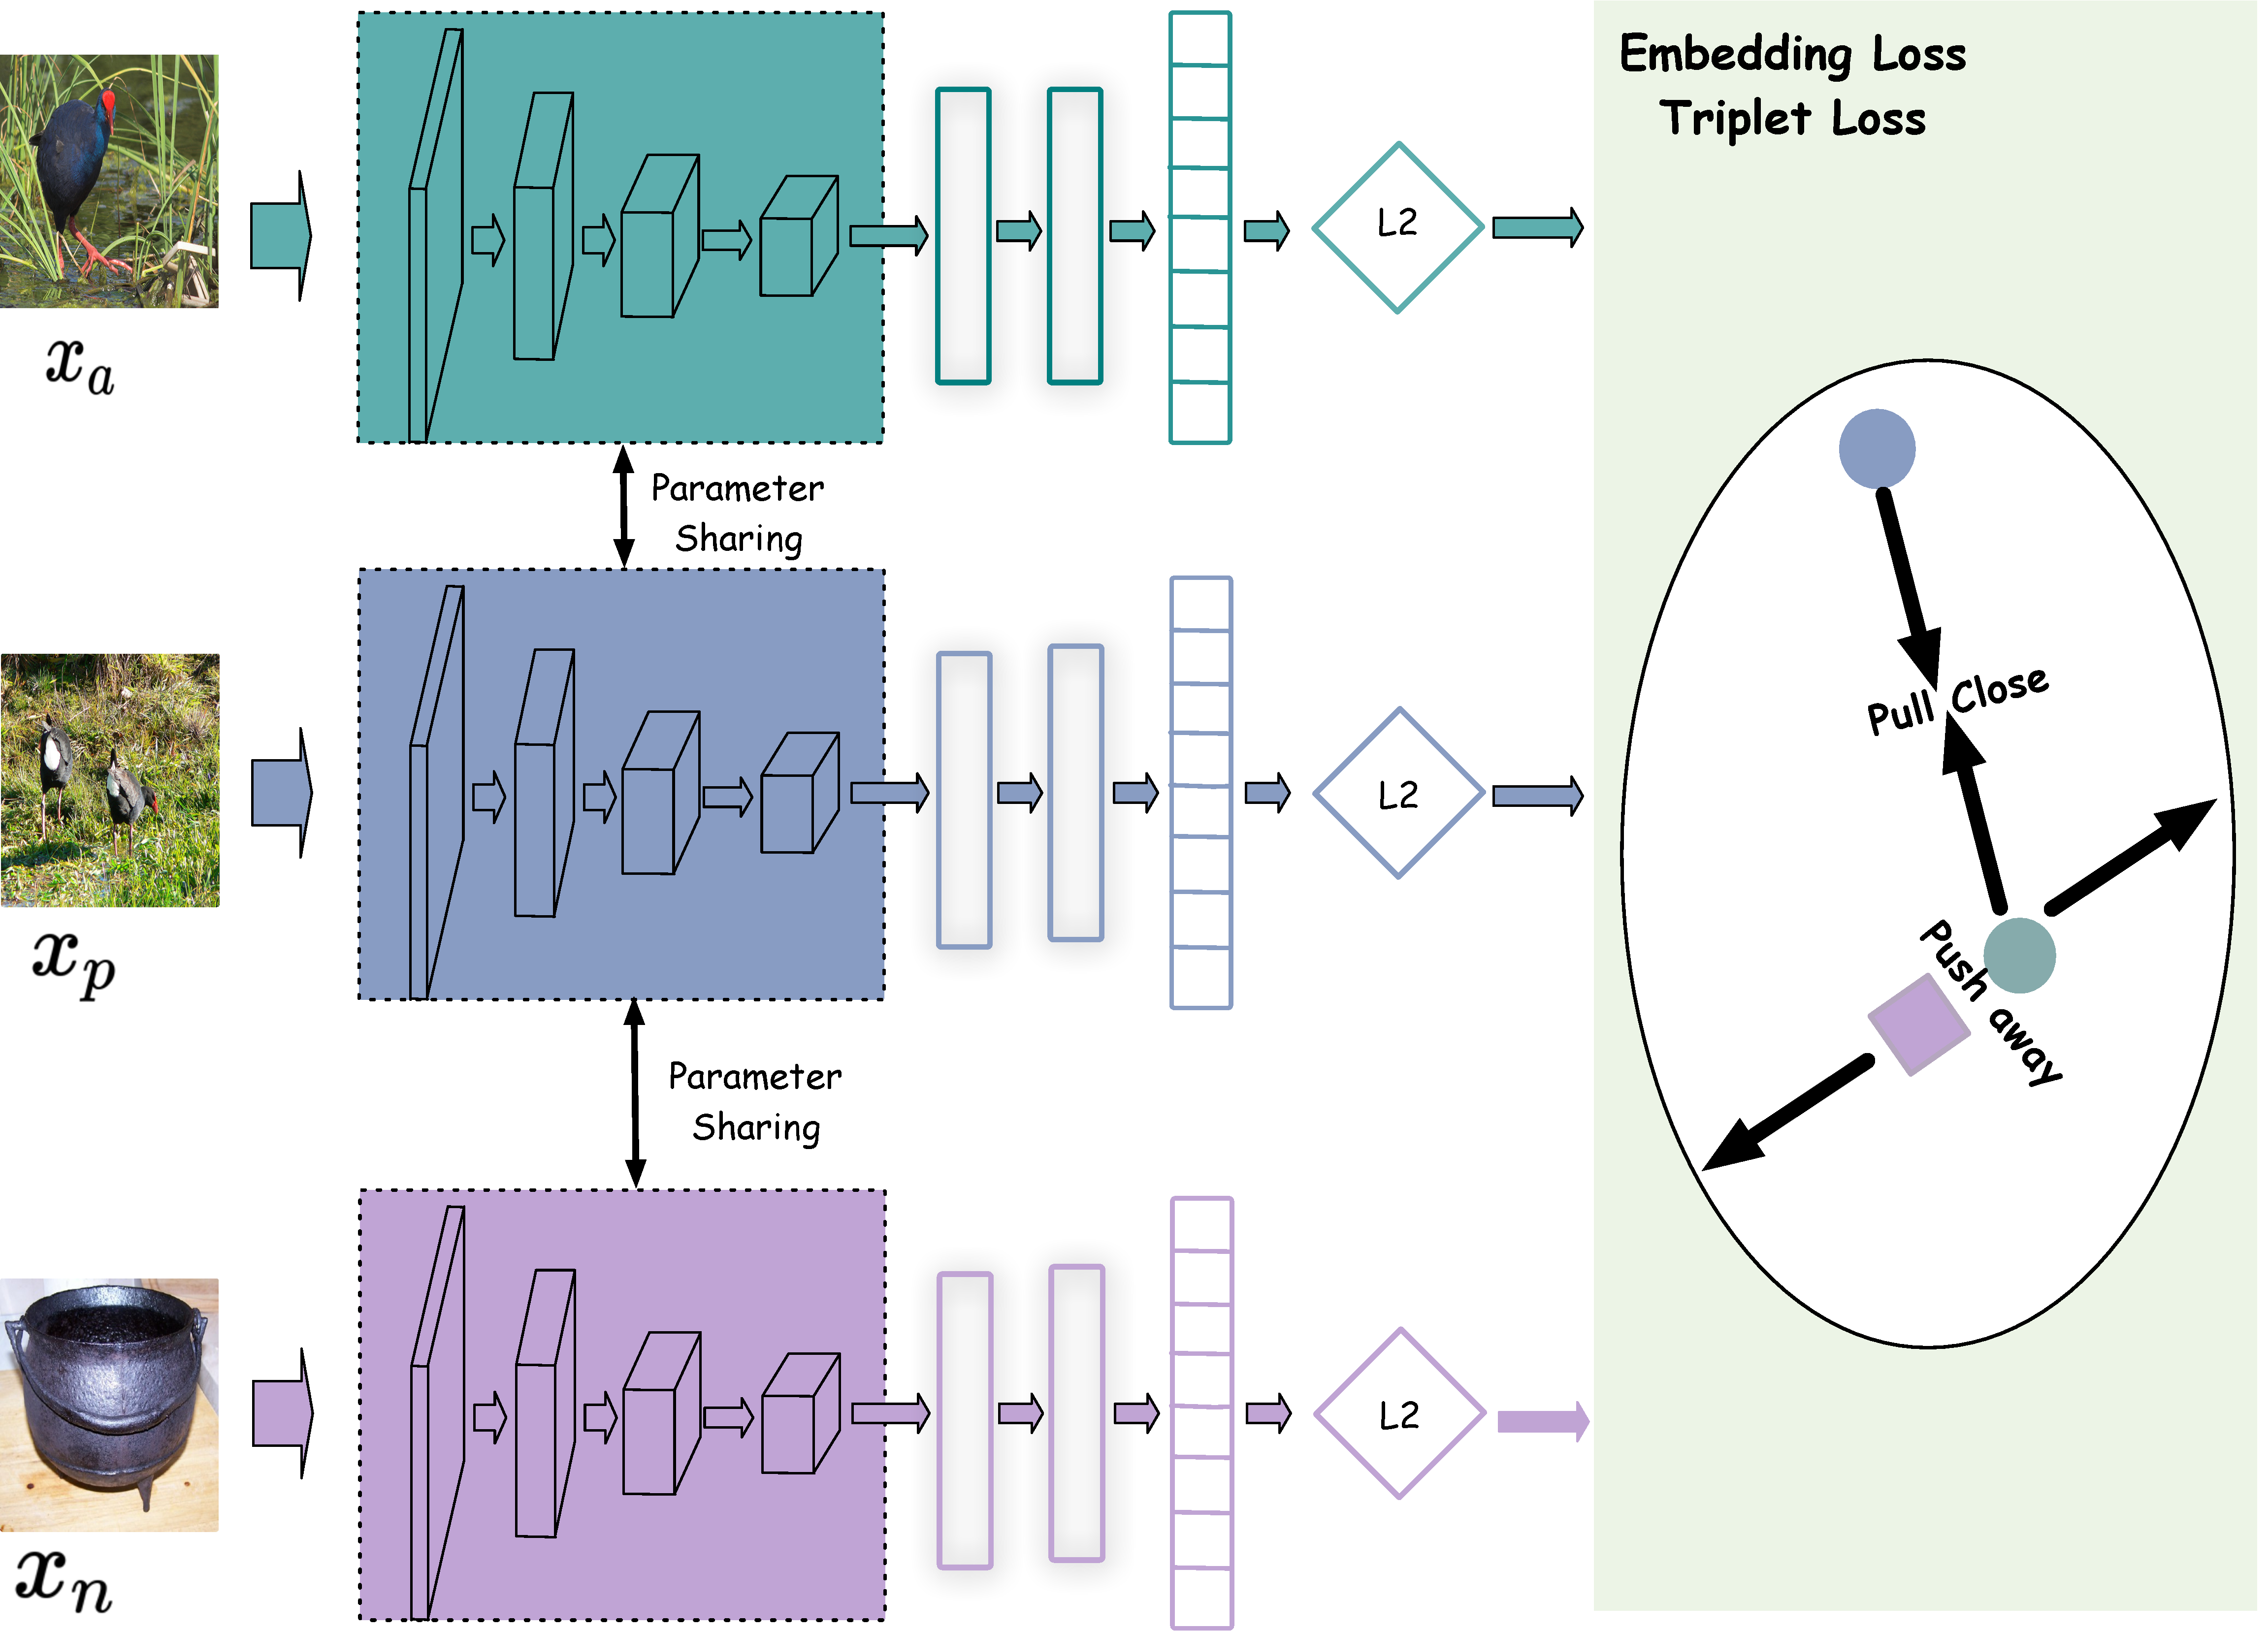
\includegraphics[width=15cm]{tripletnet.pdf} \\
    \bicaption[基于三元神经网络的检索方法]
      {基于三元CNN架构的微调图像检索架构。输入的图片以三元图片组的形式同时输入权重共享的CNN中, 三元图片组包含一个基准图片, 一个正样本, 一个负样本。框架使用三元损失函数进行监督学习。}
      {The framework of triplet convolutional neural network based image retrieval with triplet loss. The input images are tuples, every tuple comprising an anchor, a positve image and a negative image. The network is trained with triplet loss in an end-to-end fashion.}
   \label{fig:tripletnet}
\end{figure}
2016年, Gordo~\cite{gordo2016deep, gordo2017end} 提出基于最早的三元卷积神经网络用于图像检索。为了学习到对于检索最重要的局部信息, 文章额外训练了Regional Proposal Network~\cite{ren2015faster}用于检测图片中的目标区域, 同时基于R-MAC进行池化生成全局匹配的特征向量。\par
2019年, Xiang~\cite{xiang2019multiple} 提出 MSCNet。 MSCNet 包含一个多显著度注意力模块(Multiple Saliency Block) 来学习卷积后的特征图的显著性掩码 (Multiple Saliency Mask)。同时, 设计了一个基于Gram 矩阵的通道敏感性的模块来学习通道维度的权重, 最后基于三元损失函数监督进行模型微调。\par
仅基于三元损失训练的检索框架可能会难以学到图片用于进行分类的识别力特征, 一系列工作开始在三元神经网络后插入一个用于分类的全连接神经网络, 并用三元损失函数和分类损失函数进行联合监督:
\begin{equation}
    \mathcal{L}_{\text {Joint }}=\lambda_1 \cdot \mathcal{L}_{\text {Triplet }}\left(x_{i, a}, x_{i, p}, x_{i, n}\right)+\lambda_2 \cdot \mathcal{L}_{C E}\left(\hat{p}_i, y_i\right).
    \label{eq:triplece}
\end{equation}
其中$L_{CE}$ 如Eq.~\ref{eq:ce}所示。一个典型基于这个框架的工作有2020年Min~\cite{min2020two}等人提出的两阶段检索框架。第一阶通过Eq.~\ref{eq:triplece}进行同时的三元损失学习以及分类学习提高模型的表征能力。第二阶段基于Regional Proposal Network的输出以及第一阶段的网络, 新设计一个 Regional Generalized Mean Poolings (RGMP) 进行池化生成全局特征, 并且使用三元损失函数重训练。\par
三元损失函数在图像检索领域取得了广泛的应用, 在许多任务上都超越仅基于分类或者成对的对比损失函数。然而, 在大数据集的场景下, 三元组的数据和数据集大小成三次方增长关系。 对所有三元组进行网络训练学习显然是不现实的任务。 2017年, Hermans~\cite{hermans2017defense} 提出一个基于挖掘难样本的三元损失函数 (hard-mining triplet loss, HMT):
\begin{equation}
    \begin{aligned}
         \mathcal{L}_{\mathrm{HMT}}(\theta ; X) &=\overbrace{\sum_{i=1}^P \sum_{a=1}^K}^{\text {all anchors }}[m+\overbrace{\max _{p=1 \ldots K} \mathcal{D}\left(f_\theta\left(x_a^i\right), f_\theta\left(x_p^i\right)\right)}^{\text {hardest positive }} \\
        & \underbrace{\left.-\min _{\substack{j=1 \ldots P \\
        n=1 \ldots K}} \mathcal{D}\left(f_\theta\left(x_a^i\right), f_\theta\left(x_n^j\right)\right)\right]_{+}}_{\text {hardest negative }}. \\
        \end{aligned}
        \label{eq:hardtri}
\end{equation}
根据如上的公式所示, 损失函数使得与anchor相距最远的正样本比与anchor相距最近的负样本的距离还有$m$的间隔。 基于挖掘难样本的三元损失函数随后在图像检索的应用上, 如行人重识别~\cite{fu2018one,luohaoreid, wang2018learning, sun2018beyond,rahimpour2017person,xu2018attention, fang2019bilinear} (person re-identification)和车辆重识别~\cite{chu2019vehicle, meng2020fine, meng2020parsing, liu2020beyond} (Vehicle Re-identification)中成为了最基础的通用的损失函数。\par
尽管基于深度特征的图像检索~\cite{wmz2021,zhq2017, zhanghao2018,mdm2014, rxl2018, cshuang2019, zhouye2017}相比于基于手工特征的检索方法取得了性能上的飞跃, 然而存储高维的实数向量特征对于大规模检索来说并不可行。现实场景下的应用图像数据库甚至可以达到千亿的级别, 这种基于实数向量特征的存储开销以及检索速度无法满足实际的需求。
\subsection{基于深度哈希的大规模检索}
为了满足超大规模图像检索对于检测速度以及存储的需求, 深度哈希技术被引入到图像检索领域。这一小节我们先介绍最近邻搜索以及近似最近邻搜索, 然后介绍了基于汉明编码以及量化编码的检索, 最后我们重点介绍了基于深度学习的哈希编码以及量化的方法进展。
\subsubsection{最近邻搜索和次最近邻搜索}
\textbf{最近邻搜索}是很多机器学习算法的基础, 旨在给定一个查询数据$q$ 在数据库$\mathcal{X}$中找到与$q$在某个距离度量下的最近的点 $NN(q)$:
\begin{equation}
    \mathrm{NN}(x)=\operatorname{argmin}_{x \in \mathcal{X}} \text{dist}(x, q).
\end{equation}
其中$\text{dist}(x, q)$ 是$x$ 和 $q$在某特定距离度量下的距离。通常对$x \in \mathbb{R}^d$, 可以使用 $l_s$ 范数, 比如 $l_2$ 即欧式距离:
\begin{equation}
    \|\mathbf{x}-\mathbf{q}\|_s=\left(\sum_{i=1}^d\left|x_i-q_i\right|^s\right)^{1 / s}.
\end{equation}
最简单的实现最近邻搜索的方法是暴力遍历搜索, 但是由于暴力遍历的计算复杂度是$O(d|\mathcal{X}|)$, 无法扩展到大规模检索的场景。对于低维数据的最近邻检索常用的还有 KD-Tree~\cite{friedman1977algorithm}, 可是当数据的维度较大时, KD-Tree 会退化成遍历搜索, 甚至性能会低于暴力搜索。 \par
\textbf{近似最近邻搜索}是指以较大概率找到最相近的点,而不是完全精确的找到最近的点。对于$1 + \epsilon$ 近似最近邻搜索的正式定义为: 给定一个$q$, 从数据库中找到一个数据点满足:
\begin{equation}
    \text{dist}(q, x) \leq (1 + \epsilon)\text{dist}(q, x^*). 
\end{equation}
其中 $x^* = NN(q)$是真正的最近邻。常见的近似最近邻搜索方法可以分成三类: 基于哈希编码的方法~\cite{weiss2008spectral,weiss2012multidimensional,xu2013harmonious, salakhutdinov2009semantic, indyk1998approximate}, 基于量化的方法~\cite{jegou2010product, kalantidis2014locally, chen2010approximate, ge2013optimized} 以及基于图的方法~\cite{hajebi2011fast, malkov2014approximate, malkov2018efficient}。在本文中, 我们主要讨论前两种方法的应用。
\subsubsection{哈希编码}
基于哈希编码的近似最近邻方法将高维的数据映射压缩到一个低维的二进制向量, 也就是哈希码。 在图像检索中, 基于哈希的方法学习一个哈希函数 $h(.)$  将图片数据$x$转换成为 $K$ 个比特的二进制编码 $b$:
\begin{equation}
    h(x) = \text{sgn}(f(W^Tx + b)).
\end{equation}
其中 $f(.)$ 是一个任意的映射函数。$sgn(.)$ 是符号函数:
\begin{equation}
    \operatorname{sgn} (x) := \begin{cases}-1 & \text { if } x \leq 0,  \\ 1 & \text { if } x>0. \end{cases}
\end{equation}
$\operatorname{sgn} $将连续的向量二值化变成二进制哈希编码。经过$h(.)$ 得到的哈希编码需要保留图片$x$的视觉相似性, 通过这样的方式, 原始图片的相似度可以通过得到的哈希编码的相似度进行刻画。在哈希编码常用的距离是汉明距离 (Hamming Distance):
\begin{equation}
    \mathcal{D}_h(b_i, b_j) = \sum_{k = 1}^{K} \delta \left[b_{ik} \neq b_{jk} \right].
\end{equation}
其中$K$是哈希编码的长度。汉明距离刻画了两个哈希码$b_i$和$b_j$的不同位的总量。 如果哈希码的取值是$\left\{0, 1 \right\}$, 则两个哈希码的距离也等于:
\begin{equation}
    \mathcal{D}_h(b_i, b_j)=\left\|b_i - b_j\right\|_1.
\end{equation}
如果哈希码的取值是 $\left\{-1, 1\right\}$, 则汉明距离也等于:
\begin{equation}
    \mathcal{D}_h(b_i, b_j)= \frac{1}{2} \left ( K - b_i^Tb_j \right ).
\end{equation}
汉明距离的计算可以用逐位的 xor 指令计算, 比基于实值向量的欧式距离速度显著快很多。
对于哈希码的近似邻搜索方法一般有两种: \textbf{哈希查表法} (Hash Table Lookup) 和 \textbf{哈希码排序} (Hash Code Ranking)。 基于\textbf{哈希查表法}的搜索把哈希码一致的图片存在同一个哈希桶中。搜索时, 取出$q$对应哈希码所在的哈希桶中的所有图片。如果存储的是高维向量, 还可以将取出的高维向量重新计算欧式距离进行再排序。同时, 为了提高检索的召回率(recall), 一般也可以选取多个和检索的哈希码相近的哈希桶里的所有数据。 基于\textbf{哈希码排序}的方法则是直接将$q$对应的哈希码与数据库中所有的哈希码进行汉明距离计算, 然后进行排序。由于汉明距离的计算可以使用xor进行加速, 以及哈希码的存储开销远低于实值的向量, 这种方式虽然也是 $O(\left|\mathcal{X} \right|)$, 也可以在实际中被采用。 同时为了加快搜索速度, 传统基于倒排索引(Inverted Index)的加速方法也可以使用。 \par
传统基于哈希编码的图像检索方法, 一般包含两个步骤: \textbf{基于手工特征提取}: 是用如基于全局特征提取的方法 GIST或者SIFT这种全局特征提取的方法得到特征表征向量。\textbf{哈希函数学习}: 学习一个哈希函数把标签一致的特征向量映射成接近的哈希码, 典型的方法有 Locality Sensitive hashing~\cite{charikar2002similarity}, Spectral hashing~\cite{weiss2008spectral}, ICA hashing~\cite{he2011compact}, LDAHash~\cite{strecha2011ldahash}, Spec hashing~\cite{lin2010spec}, Spherical hashing~\cite{heo2012spherical}。
\subsubsection{量化编码}
\begin{figure}[!htp]
    \centering
    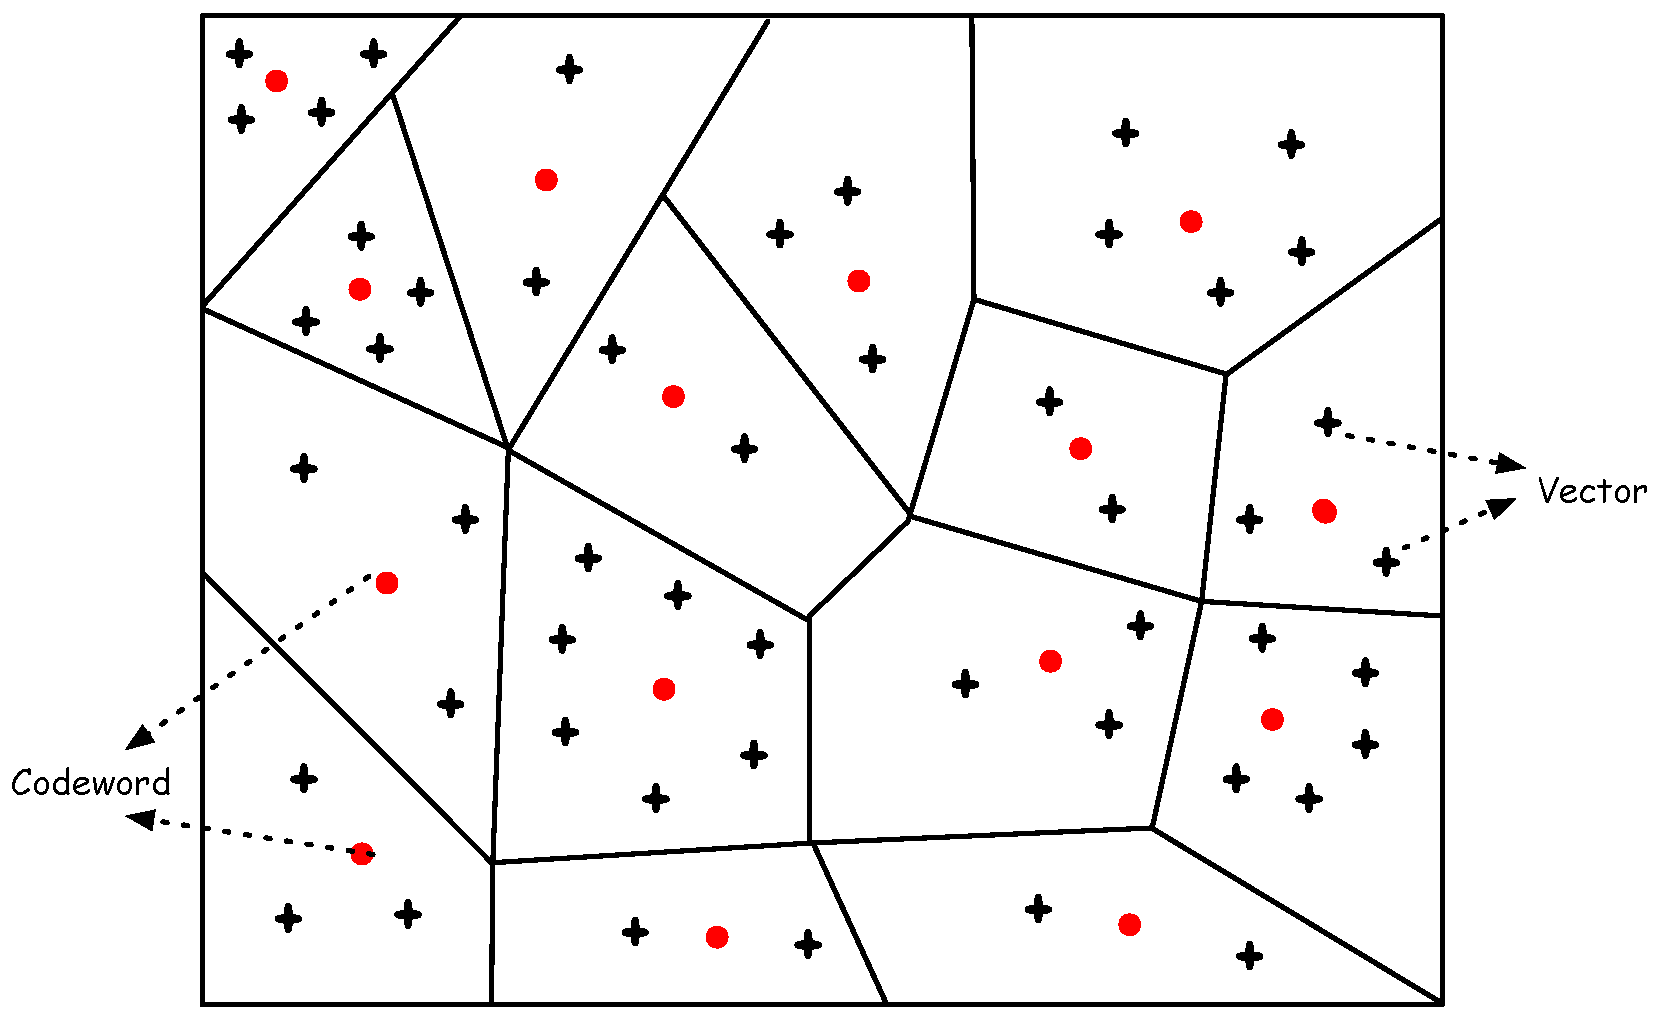
\includegraphics[width=14cm]{vq.pdf} \\
    \bicaption[向量量化的示意图]
      {二维空间的向量量化示意图。黑色的+ 代表着输入向量, 红色的点代表着codeword, 被线分隔的代表者每个沃罗诺伊室。}
      {The illustration of vector quantization in two-dimensional space. The black + denotes the input vector while the red circle represents the codeword. Cells separated by black lines are called voronoi cells. }
   \label{fig:vectorquant}
\end{figure}
基于量化编码的哈希方法是近似邻搜索的另一个主要的研究方向。一个经典的量化方法是\textbf{向量量化} ~\cite{gray1984vector}是把特征空间离散成多个码字, 然后通过把向量映射成对应码字的索引进行压缩编码, 简单示意图如 Fig.~\ref{fig:vectorquant}。量化方法中最重要的是一个量化器 (quantizer)  $q$ 是一个函数,将一个 D 维的向量 $x \in \mathbb{R}^D$映射到另一个有限的向量集中的一个向量:
\begin{equation}
    q(x) \in \mathcal{C} = \left \{ c_i; i \in  \mathcal{I}\right\}.
    \label{eq:vector}
\end{equation}
其中 $\mathcal{I} = 0 .... k-1$ 是一个有限的索引的集合。$c_i$ 叫做centroid或者叫做codeword。  而包含所有$k$个codeword的集合$\mathcal{C}$叫做codebook。 quantizer也可以换一种表述为$q(x) = d(e(x))$。 其中$e(.)$ 叫做 encoder, 把输入映射到一个索引$i$。 而 $d(i)$叫做decoder, 将索引$i$恢复成对应的codeword $c_i$。 所有的被映射到同一个索引$i$ 的原始向量的集合 $\mathcal{V}_i$叫做沃罗诺伊室 (voronoi cell):
\begin{equation}
    \mathcal{V}_i \triangleq\left\{x \in \mathbb{R}^D: q(x)=c_i\right\}.
\end{equation}
Quantizer的质量评估一般是由以下决定:
\begin{equation}
    E=\frac{1}{n} \sum_{\mathbf{x}}\|\mathbf{x}- d(e(x))\|^2.
\end{equation}
其中$E$也叫做量化误差 (Quantization Error)。\par
基于向量量化的方法应用于高维数据有一个较大的缺陷。为了实现较小的量化误差, 需要巨量的centroids来对空间进行划分。 例如对 $64$位的量化编码, centroids的数量为 $k = 2^{64}$。学习这个quantizer需要巨量的数据, 同时假如存储一个centroid消耗2kb, 则存储所有的centroids需要$2^{45}$ GB的存储, 无法在现实大规模数据中使用。 2015年, J´egou等人提出\textbf{乘积量化}很好的解决了这个问题。\par
在\textbf{乘积量化} (Product Quantization, PQ)中对于一个D维的向量$x \in \mathbb{R}^D$, 可以视为$M$个子向量的连接: $x = \left[ x^1,...x^m,...x^M \right]$。我们假设每个子向量$x^m$维度一致为$D/M$。在\textbf{乘积量化}中的quantizer $q(x) = \left[ q(x^1),...q(x^m),...q(x^M) \right]$, 其中 $q(x^m)$等同于向量量化中的quantizer, 如Eq.~\ref{eq:vector}。codebook 则是$M$个sub-codebook的笛卡尔乘积 $\mathcal{C} = \mathcal{C}^1 \times ... \times \mathcal{C}^M$。 每个codeword $c \in \mathcal{C}$则是$M$个sub-codeword的拼接 $c = \left[ c^1,...c^m,...c^M\right]$, 每个$c^m \in \mathcal{C}^m$。 对于乘积量化的量化误差定义为:
\begin{equation}
    \begin{aligned}
        & \min _{\mathcal{C}^1, \ldots, \mathcal{C}^M} \sum_{\mathbf{x}}\|\mathbf{x}-d(e(\mathbf{x}))\|^2, \\
        & \text { s.t. } \quad \mathbf{c} \in \mathcal{C}=\mathcal{C}^1 \times \ldots \times \mathcal{C}^M .
        \label{eq:pq}
        \end{aligned}
\end{equation}
其中encoder $e(.) = \left[ e^1(x^1) ,..., e^M(x^M)\right]$, 而每个子encoder $e^m$的计算如下式:
\begin{equation}
    e^m\left(\mathbf{x}^m\right)=\underset{k \in\{1, \ldots, K\}}{\arg \min }\left\|\mathbf{x}^m-c_k^m\right\|_2^2.
\end{equation}
Decoder $d(.)$则通过每个子encoder得到的索引,找到对应的sub-codeword并且进行拼接。这样原问题Eq.~\ref{eq:pq}可以通过解决多个子问题来解决, 而每个子问题则可以用k-means聚类进行计算求解。 \par
由于乘积量化编码 PQ-code 包含 $M$个 1到k的整数索引, 所以PQ-code的存储消耗为$M\log_2K$ 比特。如果用32比特的PQ-code来存储128维度的浮点32位的实值特征向量, 则内存占用量只为原来128分之1。对于乘积量化编码的距离计算, 一般采取``非对称距离计算'' (Asymmetric Distance Computation, ADC)。对于一个查询的向量 $y$ 和数据库中的向量$x$和 $x$ 经过quantizer 重建的向量$\tilde{x}$, 非对称距离$\hat{\mathcal{D}}$计算如下所示:
\begin{equation}
    \mathcal{D}(\mathbf{y}, \mathbf{x})^2 \approx \tilde{\mathcal{D}}(\mathbf{y}, \mathbf{x})^2=d(\mathbf{y}, \tilde{\mathbf{x}})^2.
\end{equation}
为了加速ADC的计算通常会通过存储距离表(Lookup Table)然后再读取距离。对于每一个查询向量$y$, 对于其每一个子向量$y^m \in \mathbb{R}^{\frac{D}{M}} (m \in \left \{ 1,...,M  \right \})$。我们计算它与对应的sub-codebook里面的所有$K$个sub-codeword $c_k^m \in \mathcal{C}$的距离, 然后将其存储在距离查找表中:
\begin{equation}
    A(m, k)=d\left(\mathbf{y}^m, \mathbf{c}_k^m\right)^2
\end{equation}
之后对于$q$和每一个检索的向量$x$的非对称距离可以通过以下得到:
\begin{equation}
    \begin{aligned}
        \tilde{\mathcal{D}}(\mathbf{y}, \mathbf{x})^2 & =\mathcal{D}(\mathbf{y}, \tilde{\mathbf{x}})^2 \\
        & =\sum_{m=1}^M \mathcal{D}\left(\mathbf{y}^m, \mathbf{c}_{i^m}^m\right)^2=\sum_{m=1}^M A\left(m, i^m\right)
    \end{aligned}
\end{equation}
其中$\mathcal{D}$是欧式距离。其中 $i = \left[i^1,...,i^M \right]$ 是 $x$对应的PQ-code。通过这种方式,只需要计算查找表$A$里的距离, 其余的距离计算如上可以通过查表解决。计算复杂度为$O(DK + MN)$, 其中$D$ 为向量的维度, $K$ 是sub-codebook的大小, $M$是sub-codebook的个数, $N$是数据库存储的数据的数量。同时PQ也可以和倒排索引等方法组合, 缩小搜索空间,提高检索效率。随后, 基于乘积量化的改进还有 optimizied product quantization~\cite{ge2013optimized}、additive quantization~\cite{martinez2016revisiting}、compositive quantization~\cite{zhang2014composite}, 以及 Iterative Quantization~\cite{gong2012iterative}。\par
基于传统哈希编码的图像检索方式由于需要先通过手工特征提取的方法提取特征,  然后通过哈希编码或者量化编码的方法压缩特征并且加速检索。由于传统手工特征提取的方式很捕捉高级语义特征, 基于深度学习的哈希检索方法成为了大规模图像检索的主流。

\subsubsection{基于深度学习的哈希}
\begin{figure}[!htp]
    \centering
    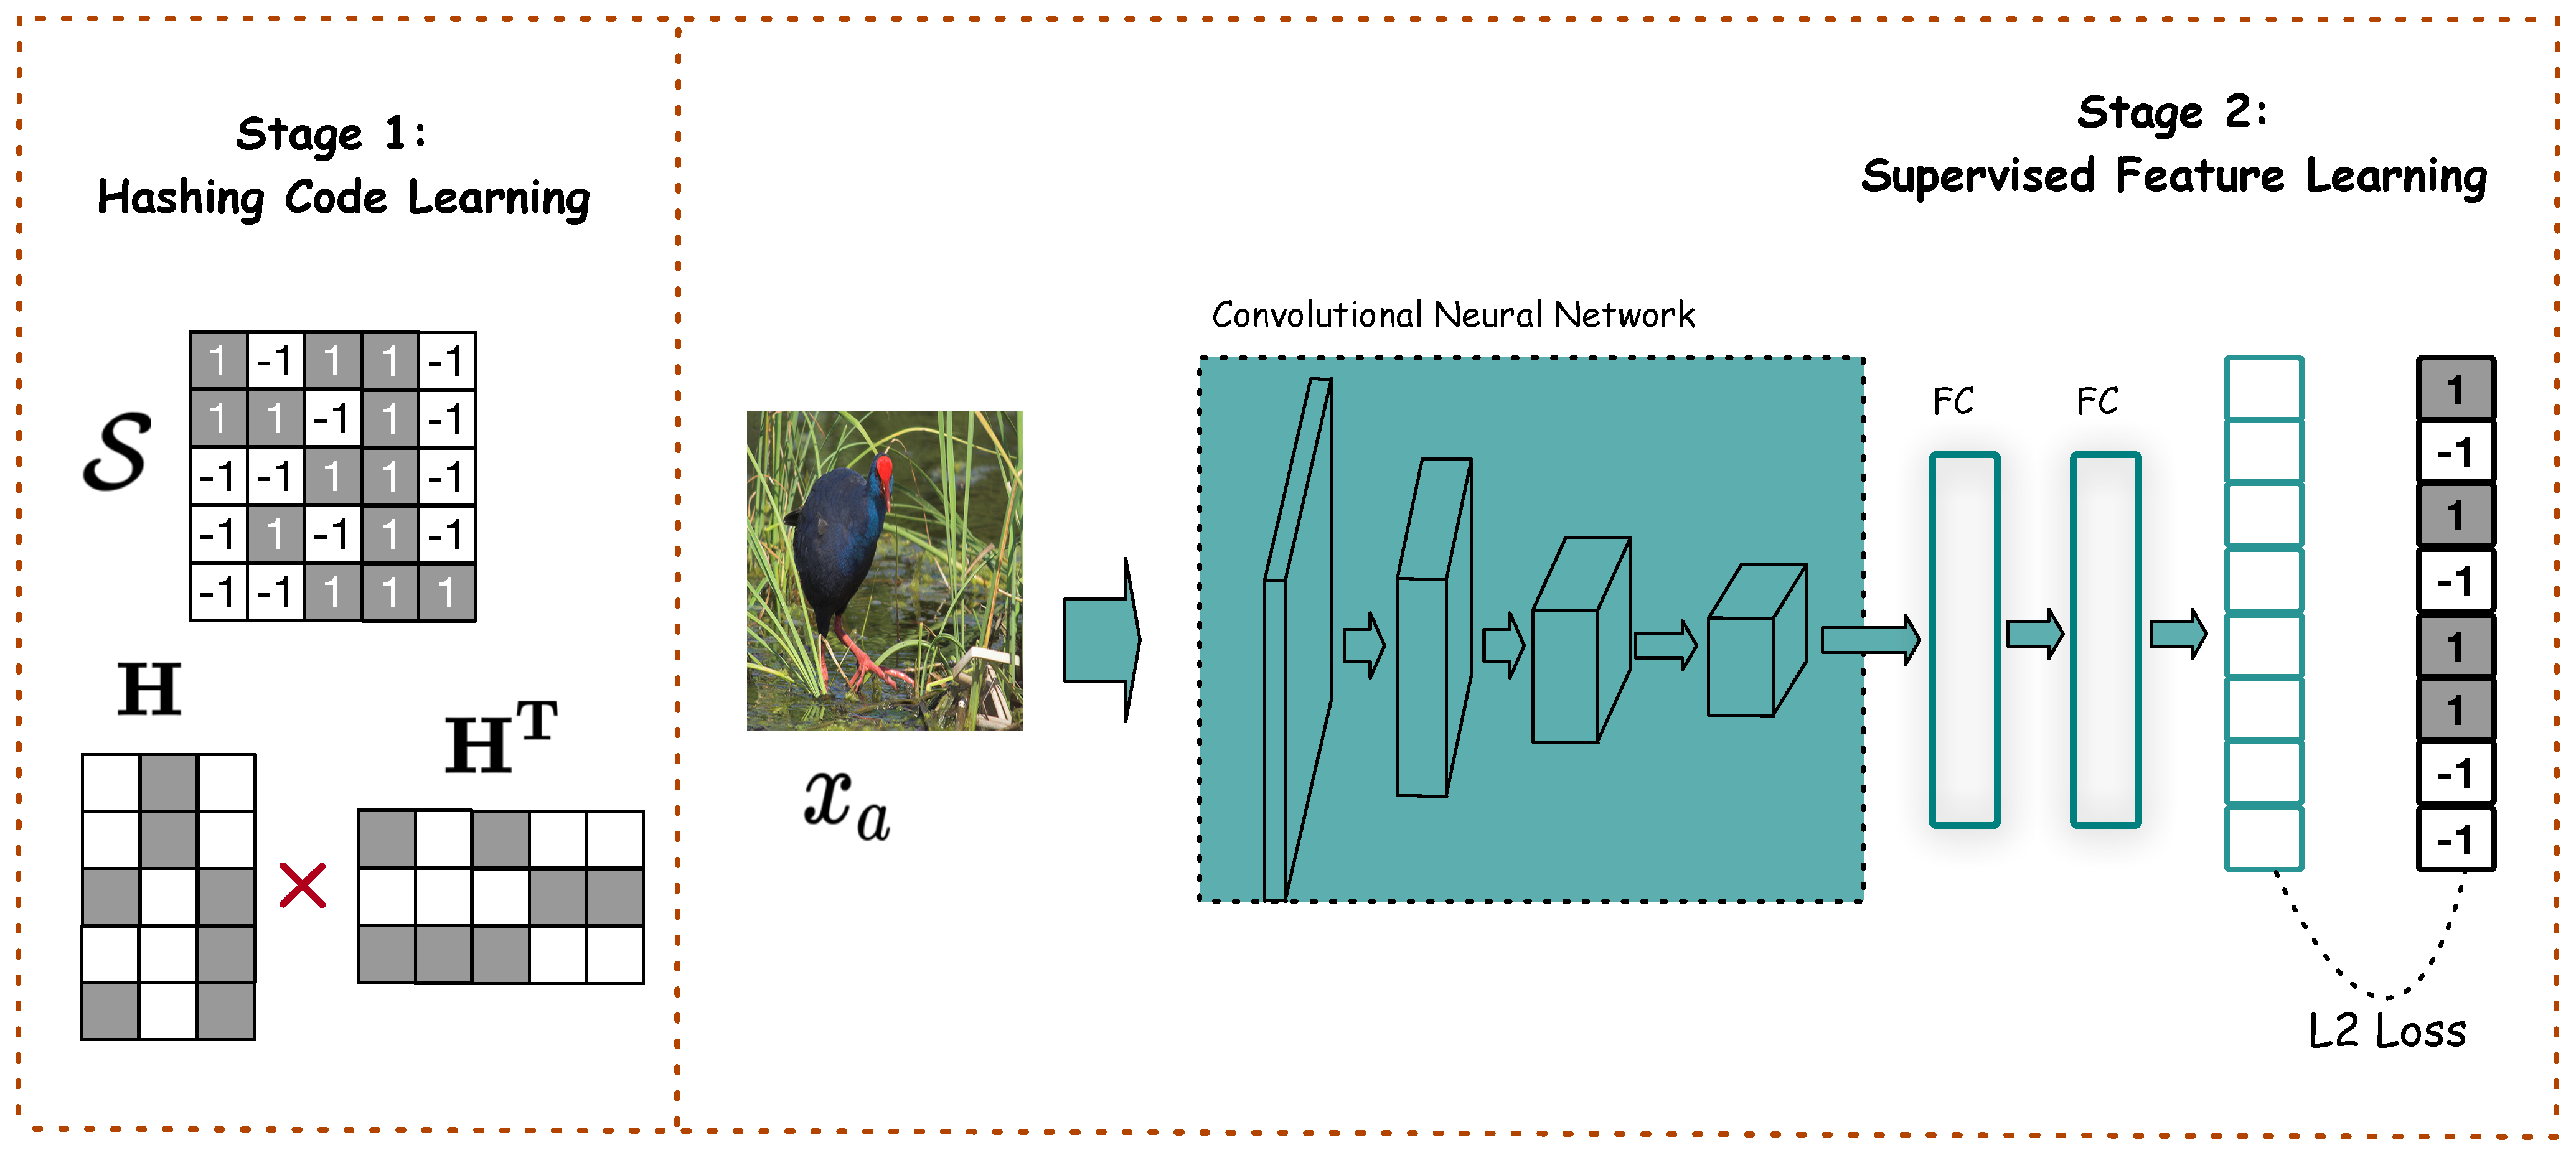
\includegraphics[width=14cm]{twoshash.pdf} \\
    \bicaption[二阶段深度哈希框架]
      {基于二阶段的深度哈希框架。第一阶段根据相似度矩阵$\mathcal{S}$学习对应的每张图片的哈希码$\mathcal{H}_i$。 第二阶段使用学习到的哈希码来监督训练卷积神经网络。}
      {The deep hashing framework based on a two-stage hashing paradigm. In the first stage, the hashing code $H_i$ is learned given the similarity matrix $\mathcal{S}$. In the second stage, the learned hashing codes are used the supervise the convolutional neural network to ouput hashing codes in an end-to-end fashion.  }
   \label{fig:twoshash}
\end{figure}

早期的基于深度学习的哈希架构是包含两个阶段,如图所示 Fig.~\ref{fig:twoshash}。 第一阶段先学习二进制哈希码,第二阶段再使用学习到的哈希码来监督训练神经网络提取特征。\par
2014年, Xia~\cite{xia2014supervised}提出第一个基于深度学习的哈希框架。第一阶段通过建立一个$n \times q$的二进制矩阵$H$, 其中第$k$行 $H_k \in \left \{ -1, 1 \right \}$。 $H_k$代表图片$I_k$的二进制哈希码。$S$是相似度矩阵, $S_{ij} = 1$如果图片$I_i$和$I_j$是语义一致的图片对, 相反的话 $S_{ij} = -1$。通过优化一下的目标函数来求解哈希矩阵$H$:
\begin{equation}
    \min _H \sum_{i=1}^n \sum_{j=1}^n\left(S_{i j}-\frac{1}{q} H_i . H_{j .}^T\right)^2=\min _H\left\|S-\frac{1}{q} H H^T\right\|_F^2.
\end{equation}
其中$\left\| . \right\|$是Frobeniusf范数。第二阶段, 通过神经网络如图所示, 在神经网络后层增加全连接层通过第一阶段学习到的哈希码监督学习神经网络的特征提取。 \par

2015年, Lai~\cite{lai2015simultaneous}提出了第一个端到端的深度哈希框架如图所示。这个框架把特征提取到哈希码的生成集合在一个深度神经网络中, 通过一个三元损失函数监督学习:
\begin{equation}
    \begin{aligned}
        & \ell_{\text {triplet }}\left(\mathcal{F}(I), \mathcal{F}\left(I^{+}\right), \mathcal{F}\left(I^{-}\right)\right) \\
        = & \max \left(0,\left\|\mathcal{F}(I)-\mathcal{F}\left(I^{+}\right)\right\|_2^2-\left\|\mathcal{F}(I)-\mathcal{F}\left(I^{-}\right)\right\|_2^2+1\right) \\
        & \text { s.t. } \mathcal{F}(I), \mathcal{F}\left(I^{+}\right), \mathcal{F}\left(I^{-}\right) \in[0,1]^q.
        \end{aligned}
\end{equation}
其中$\mathcal{F}(.)$是基于深度学习的哈希函数。$\left \| . \right \|$是用来代替计算汉明距离的 $l_2$范数。同时为了使得神经网络生成的哈希码尽量分布均匀, 文章还提出一个divide-and-conquer模块来分块通过如下的阈值化函数生成哈希码:
\begin{equation}
    g(s)=\left\{\begin{array}{rr}
        0, & s<0.5-\epsilon \\
        s, & 0.5-\epsilon \leq s \leq 0.5+\epsilon \\
        1, & s>0.5+\epsilon
        \end{array}\right.
\end{equation} 
其中$s$是神经网络经过$sigmoid$函数激活的输出概率。

这个基于端到端的哈希方法在两阶段的哈希方法上取得了较显著的性能提升。随后, ~\cite{yao2016deep} 在这个架构的基础上加入了分类损失函数, 同时优化三元损失函数和分类函数来进行同步的深度特征学习和哈希码学习:
\begin{equation}
    \mathcal{L}_{\text {Class}}(\theta)=-\frac{1}{n}\left[\sum_{i=1}^n \sum_{j=1}^c I_{\left(y^i=j\right)} \log \frac{e^{\theta_j^T x^i}}{\sum_{l=1}^c e^{\theta_l^T x^i}}\right] \text {, }
\end{equation}
其中$\theta$是神经网络的参数。$y^i$是图片标签类别。\par
2016年, Liu~\cite{liu2016deep}提出使用基于对比损失的哈希方法。为了将二值的限制条件加入神经网络中学习, 作者新增了一个量化损失函数:
\begin{equation}
    \begin{aligned}
        L_r\left(\mathbf{b}_1, \mathbf{b}_2, y\right) & =\frac{1}{2}(1-y)\left\|\mathbf{b}_1-\mathbf{b}_2\right\|_2^2 \\
        & +\frac{1}{2} y \max \left(m-\left\|\mathbf{b}_1-\mathbf{b}_2\right\|_2^2, 0\right) \\
        & +\alpha\left(\left\|\left|\mathbf{b}_1\right|-\mathbf{1}\right\|_1+\left\|\left|\mathbf{b}_2\right|-\mathbf{1}\right\|_1\right).
        \end{aligned}
\end{equation}
其中 $\mathbf{b}$是神经网络的输出, 通过$\left \| \mathbf{b} - 1 \right \|$使得输出尽量接近二进制码。\par
随后, Zhu 等人提出DHN~\cite{zhu2016deep}基于一个贝叶斯学习框架损失函数:
\begin{equation}
    L=\sum_{s_{i j} \in \mathcal{S}}\left(\log \left(1+\exp \left(\left\langle\boldsymbol{z}_i^l, \boldsymbol{z}_j^l\right\rangle\right)\right)-s_{i j}\left\langle\boldsymbol{z}_i^l, \boldsymbol{z}_j^l\right\rangle\right).
\end{equation}
其中$\mathcal{S}$是图片的相似矩阵, $S_{ij} = 1$ 如果$I_i$和 $I_j$是语义接近的图片, 反之为0。为了降低量化损失, 作者还是用了一个使用了一个先验分布, 使得哈希码$h$在接近-1和1的时候概率尽量大:
\begin{equation}
    p\left(\boldsymbol{h}_i\right)=\frac{1}{2 \epsilon} \exp \left(-\frac{\left\|\left|\boldsymbol{h}_i\right|-\mathbf{1}\right\|_1}{\epsilon}\right).
\end{equation}

2017年, Cao等人提出HashNet~\cite{cao2017hashnet},  在DHN的基础上使用$\operatorname{tanh}(\beta z)$无限接近用于二值化神经网络输出的$\operatorname{sgn}$, 从而直接解决$sgn$不可导的问题:
\begin{equation}
    \lim _{\beta \rightarrow \infty} \tanh (\beta z)=\operatorname{sgn}(z).
\end{equation}
当逐步增大$\beta$, $\operatorname{tanh}(\beta z)$逐步接近于$sgn$。
2021年, Tu等人提出基于Partial Softmax的哈希方法, 同时训练一个特征提取的卷积神经网络和一个类别映射的神经网络, 以及一个新的 Partial Softmax损失函数来监督求解。同时, 基于域适应的哈希算法~\cite{fyw2018}, 基于注意力机制的深度哈希算法~\cite{jhj2021,cg2020}, 以及基于对抗学习的深度哈希算法~\cite{yr2021}等也取得了较好的效果。 深度哈希技术开始被应用在多个计算机视觉相关的大规模图像检索任务中~\cite{csg2020,qh2018, ljn2019 }。
\begin{figure}[!htp]
    \centering
    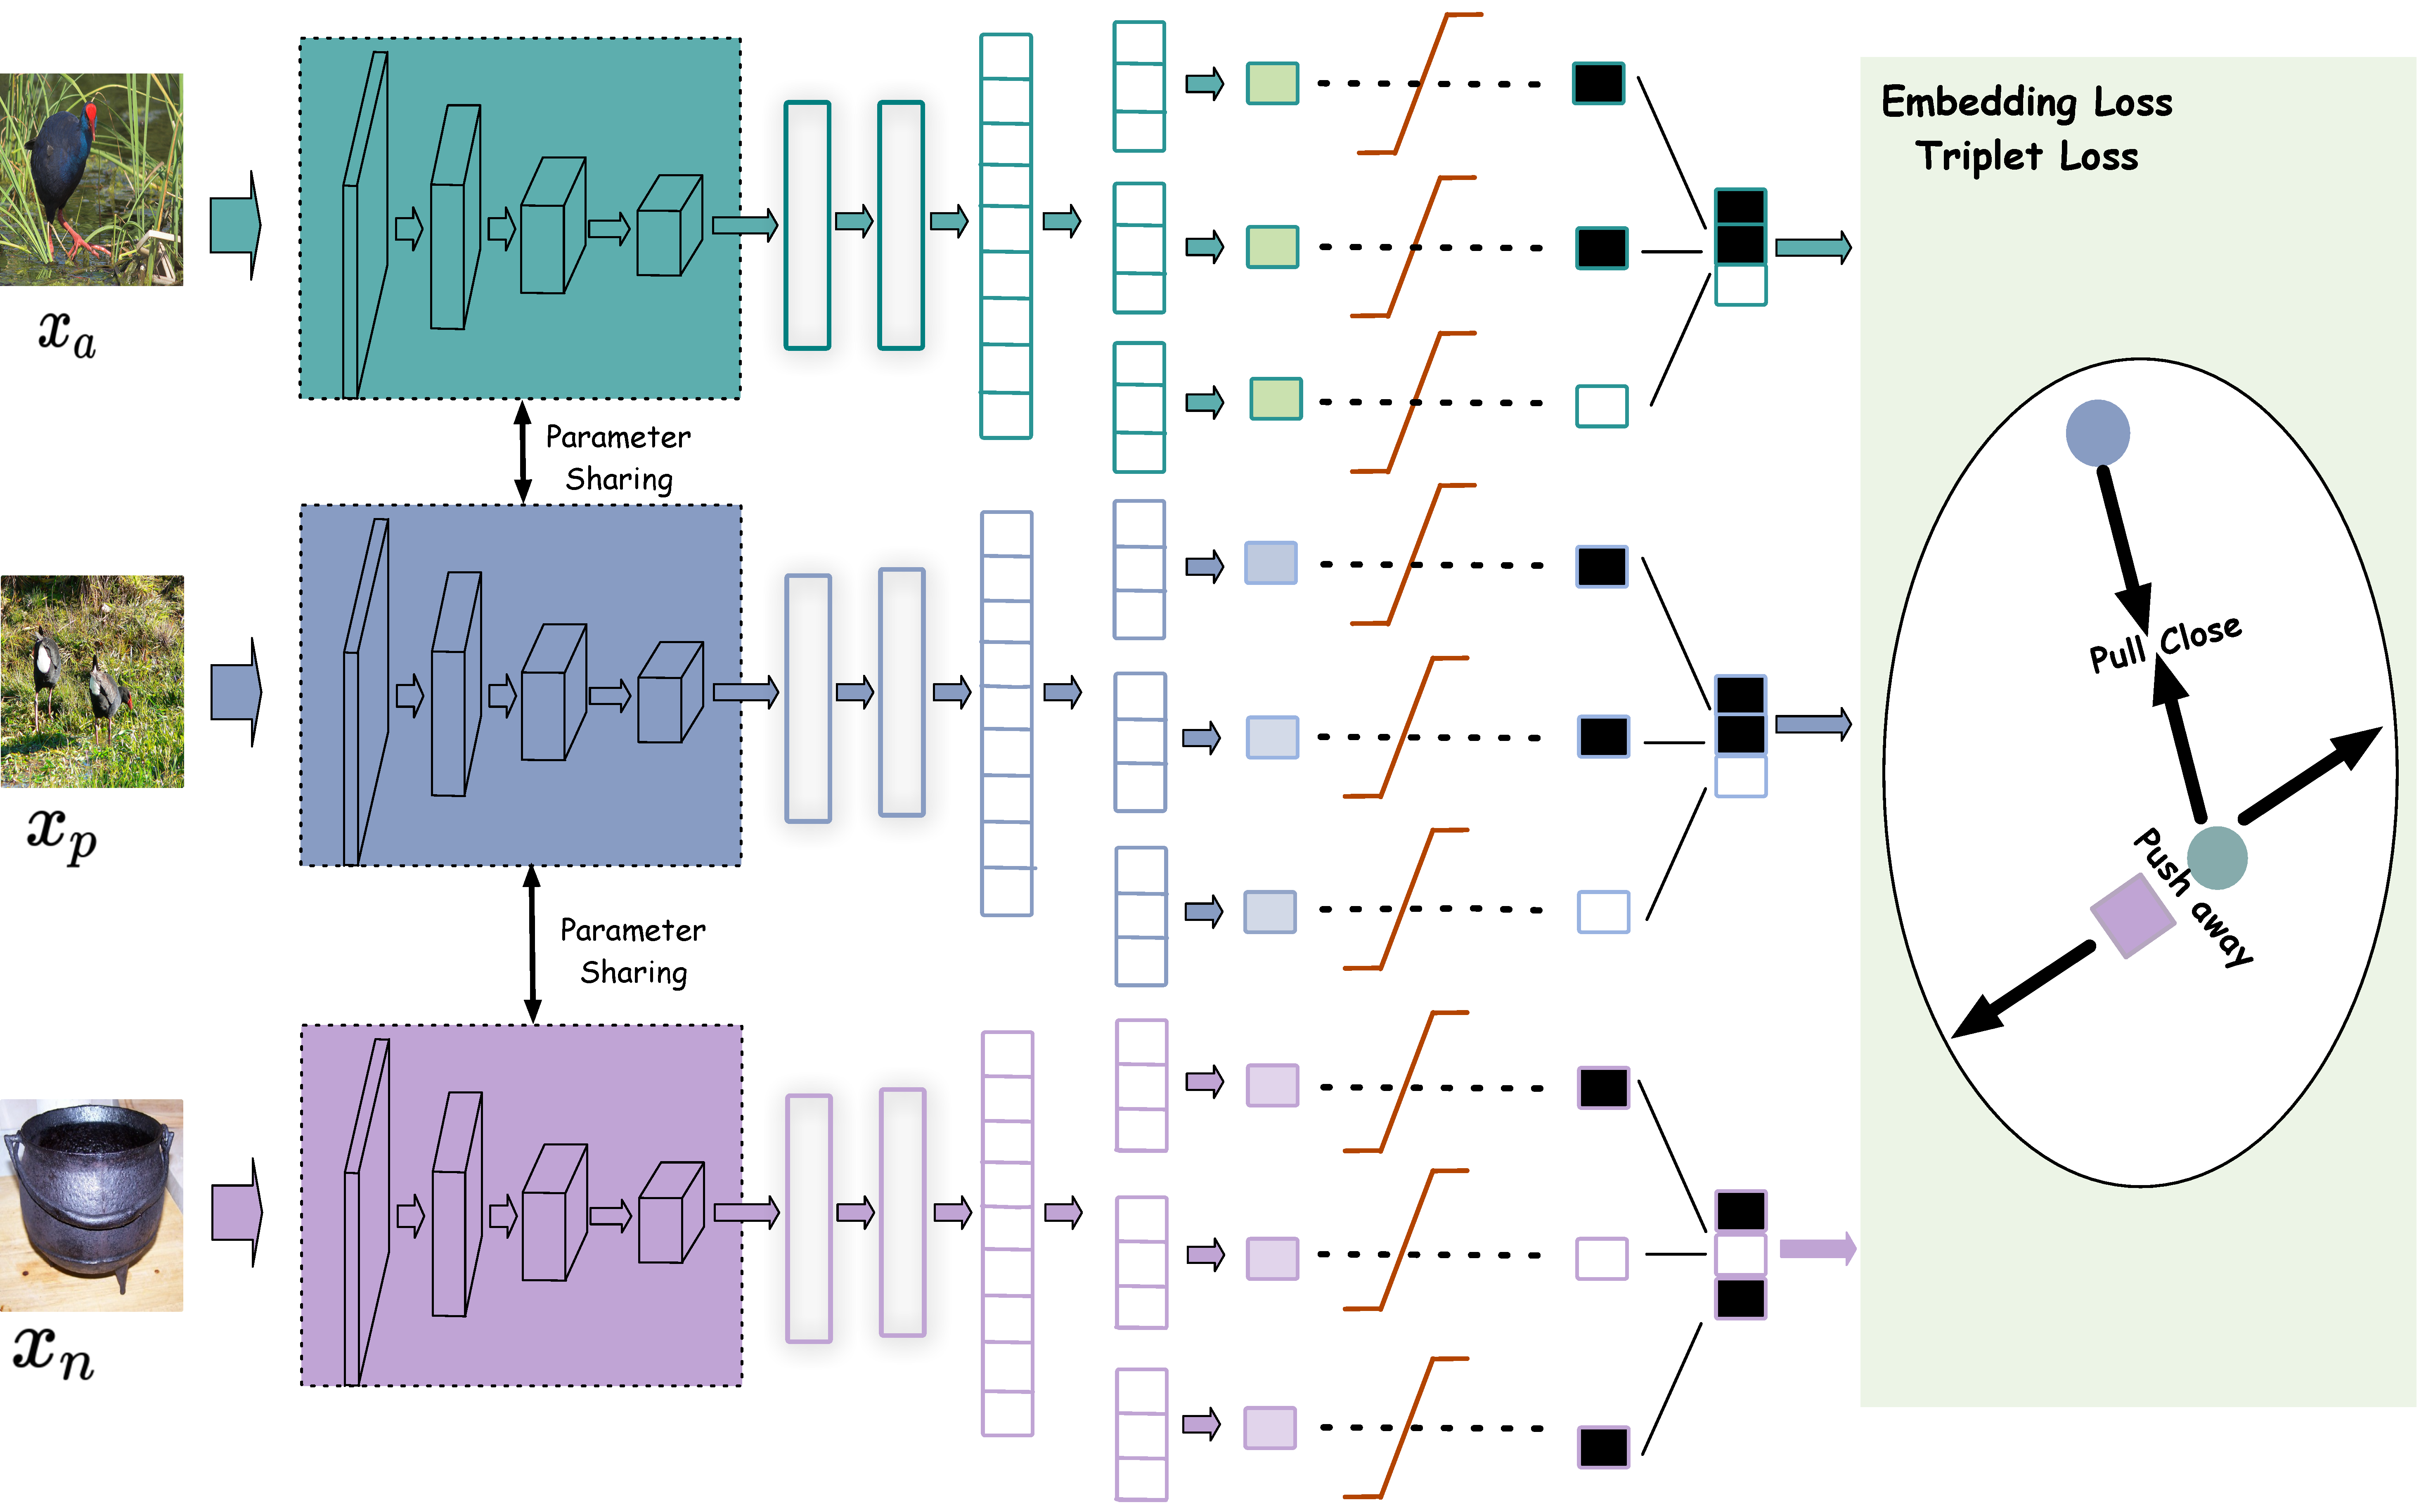
\includegraphics[width=14cm]{cnnh.pdf} \\
    \bicaption[CNNH深度哈希网络的框架图]
      {基于三元网络的深度哈希框架CNNH。输入的图片为三元组$x_a, x_p, x_n$。$x_a$为anchor图片, $x_p$ 为anchor的正样本, $x_n$为anchor的负样本。文章引入一个divide-and-encode模块, 将全连接输出向量分成多个部分, 然后分别生成哈希码。}
      {The framework of triplet-network based hashing for CNNH. The input images are organized into triplets ($x_a, x_p, x_n$) where $x_a$ is the anchor, $x_p$ is the positve image for the anchor and $x_n$ is the negative. Then, output from the fully connected layer  is fed into the divide-and-encode network to generate hash code separately and independently.}
   \label{fig:trihash}
\end{figure}
\subsubsection{基于深度学习的量化}
第一个将量化学习引入深度图片检索的工作是\textbf{DQN}~\cite{yue2016deep}, 由清华大学的Cao~等人提出, 基础架构如图~\ref{fig:dqn}所示。\textbf{DQN} 采取深度卷积神经网络以及成对的对比损失函数提取图片特征, 随后使用乘积量化(Product Quantization)来将高位特征向量压缩成二进制哈希码。其中的乘积量化损失函数如下所示:
\begin{equation}
    \begin{gathered}
        Q=\sum_{m=1}^M \sum_{i=1}^N\left\|\boldsymbol{z}_{i m}^l-\boldsymbol{C}_m \boldsymbol{h}_{i m}\right\|_2^2 \\
        \left\|\boldsymbol{h}_{i m}\right\|_0=1, \boldsymbol{h}_{i m} \in\{0,1\}^K,
        \end{gathered}
    \label{eq:pqloss}
\end{equation}
其中$\mathbf{C}=\left[\mathbf{c}_{m 1}, \ldots, \mathbf{c}_{m K}\right]$ 代表codebook, 每个codebook包含$K$个codewords。 $\mathbf{z}_i=\left[\mathbf{z}_{i 1} ; \ldots ; \mathbf{z}_{i M}\right], i=1, \ldots, n$ 并且 $\mathbf{z}_{im}$是$\mathbf{z}_i$ 在第$m$个子空间的子向量。 所有的子空间的codewords 通过k-means聚类算法学习得到。 通过最小化乘积量化损失函数$Q$, 特征向量$\mathbf{z}$ 可以被量化成对应的二进制码$b$。\par
\begin{figure}[!htp]
    \centering
    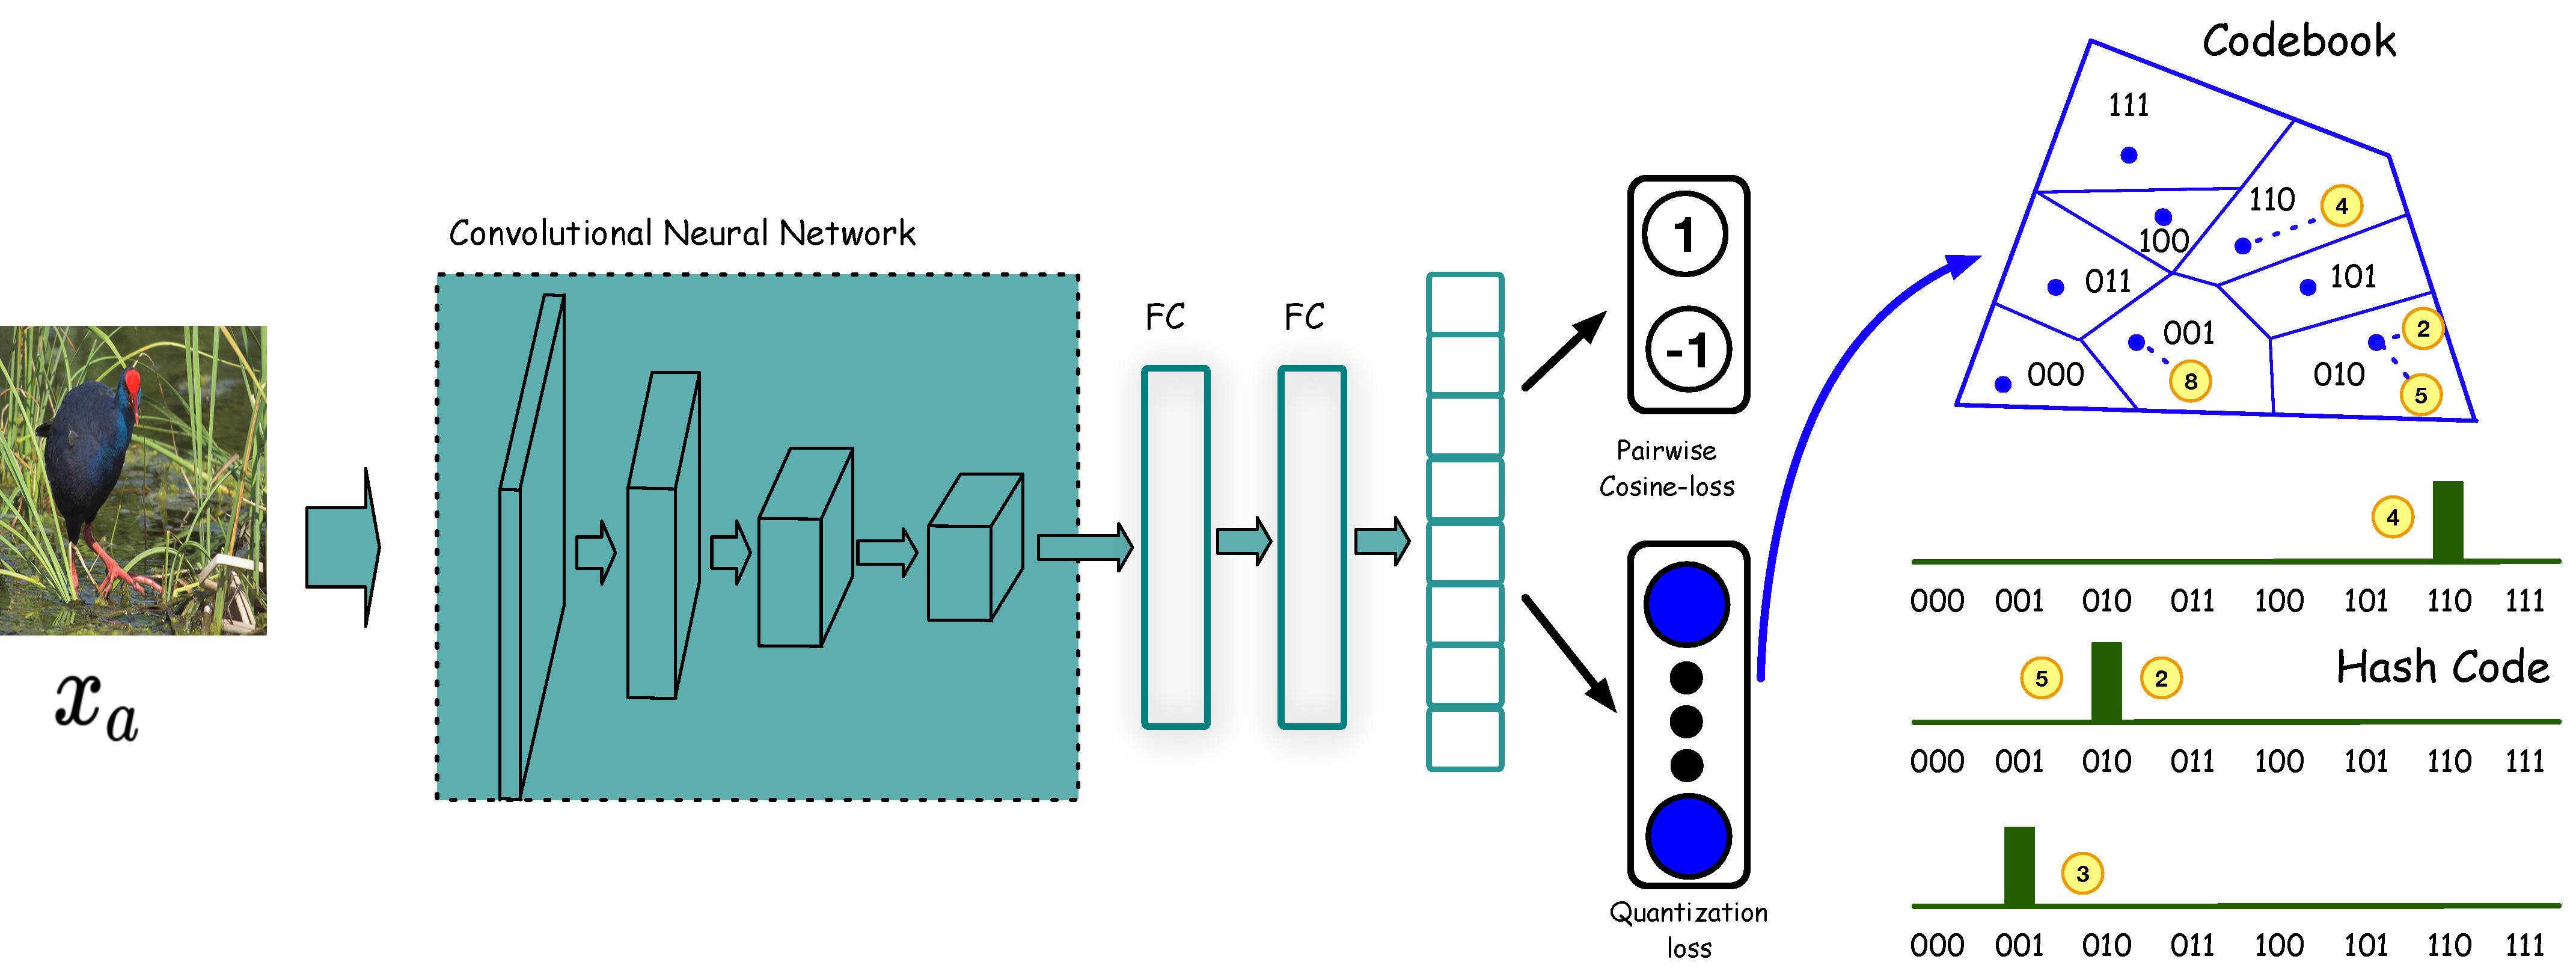
\includegraphics[width=15cm]{dqn.pdf} \\
    \bicaption[深度乘积量化的框架图]
      {深度乘积量化网络的框架图。左侧是标准的卷积神经网络用语特征提取。成对的余弦损失函数用来进行保距的度量学习。同时采用了量化损失函数用来生成紧凑的量化编码。}
      {The framework of deep quantization network for image retrieval. The left is a standard convolutional neural network for feature extraction. Pairwisie cosine loss is adopted for similarity preserving learning. Product quantization loss is further employed to generate compact binary codes.}
   \label{fig:dqn}
\end{figure}
2018年, Liu 等人提出基于三元组的乘积量化\textbf{DTQ}~\cite{liu2018deep}。作者提出一个新颖的三元组选择算法, 在每一轮训练中动态随机生成难三元组样本输入到三元卷积神经网络中进行训练。同时, 作者提出一个新颖的基于弱正交性的三元乘积量化损失函数来生成二进制编码。弱正交性的引入可以降低codebook的冗余性以及控制卷积神经网络生成的深度特征的可量化度。\par
2018, Yu ~\cite{yu2018product}等人提出乘积量化网络\textbf{PQN}来进行图像检索。不同于\textbf{DTQ}和\textbf{DQN}使用K-means算法无监督生成乘积量化编码中的每个sub-codebook中的codewords, \textbf{PQN}提出一个可导的软乘积量化层, 可以接入传统的卷积神经网络后进行端对端的训练, 同时作者还提出一个三元量化损失函数来直接监督学习深度特征以及codewords。\par
随后, 基于\textbf{PQN}, Yu~\cite{yu2018generative} 提出一个基于生成对抗网络的端到端的乘积量化网络。其架构除了传统的卷积神经网络用来提取图片特征以外还包含了一个基于DCGAN~\cite{radford2015unsupervised}的架构。通过一个生成器 (Generator) 从前者提取生成的特征中生成图片使得判别器 (Discriminator) 无法分辨真实图片和生成器生成的图片从而使得卷积神经网络提取出有判别性的图片特征, 如下所示:
\begin{equation}
    \min _{\Theta_G} \max _{\Theta_D} \log (\mathbf{D}(I))+\log \left(1-\mathbf{D}\left(I^R\right)\right), 
\end{equation}
其中 $\Theta_G$ 和 $\Theta_D$是生成器和判别器的参数。 $I$是真实的图片, $I^R$ 是生成器生成的图片。同时, 作者也基于 \textbf{PQN}将乘积量化集成到端到端的网络训练中, 并且基于三元损失函数进行监督训练:
\begin{figure}[!htp]
    \centering
    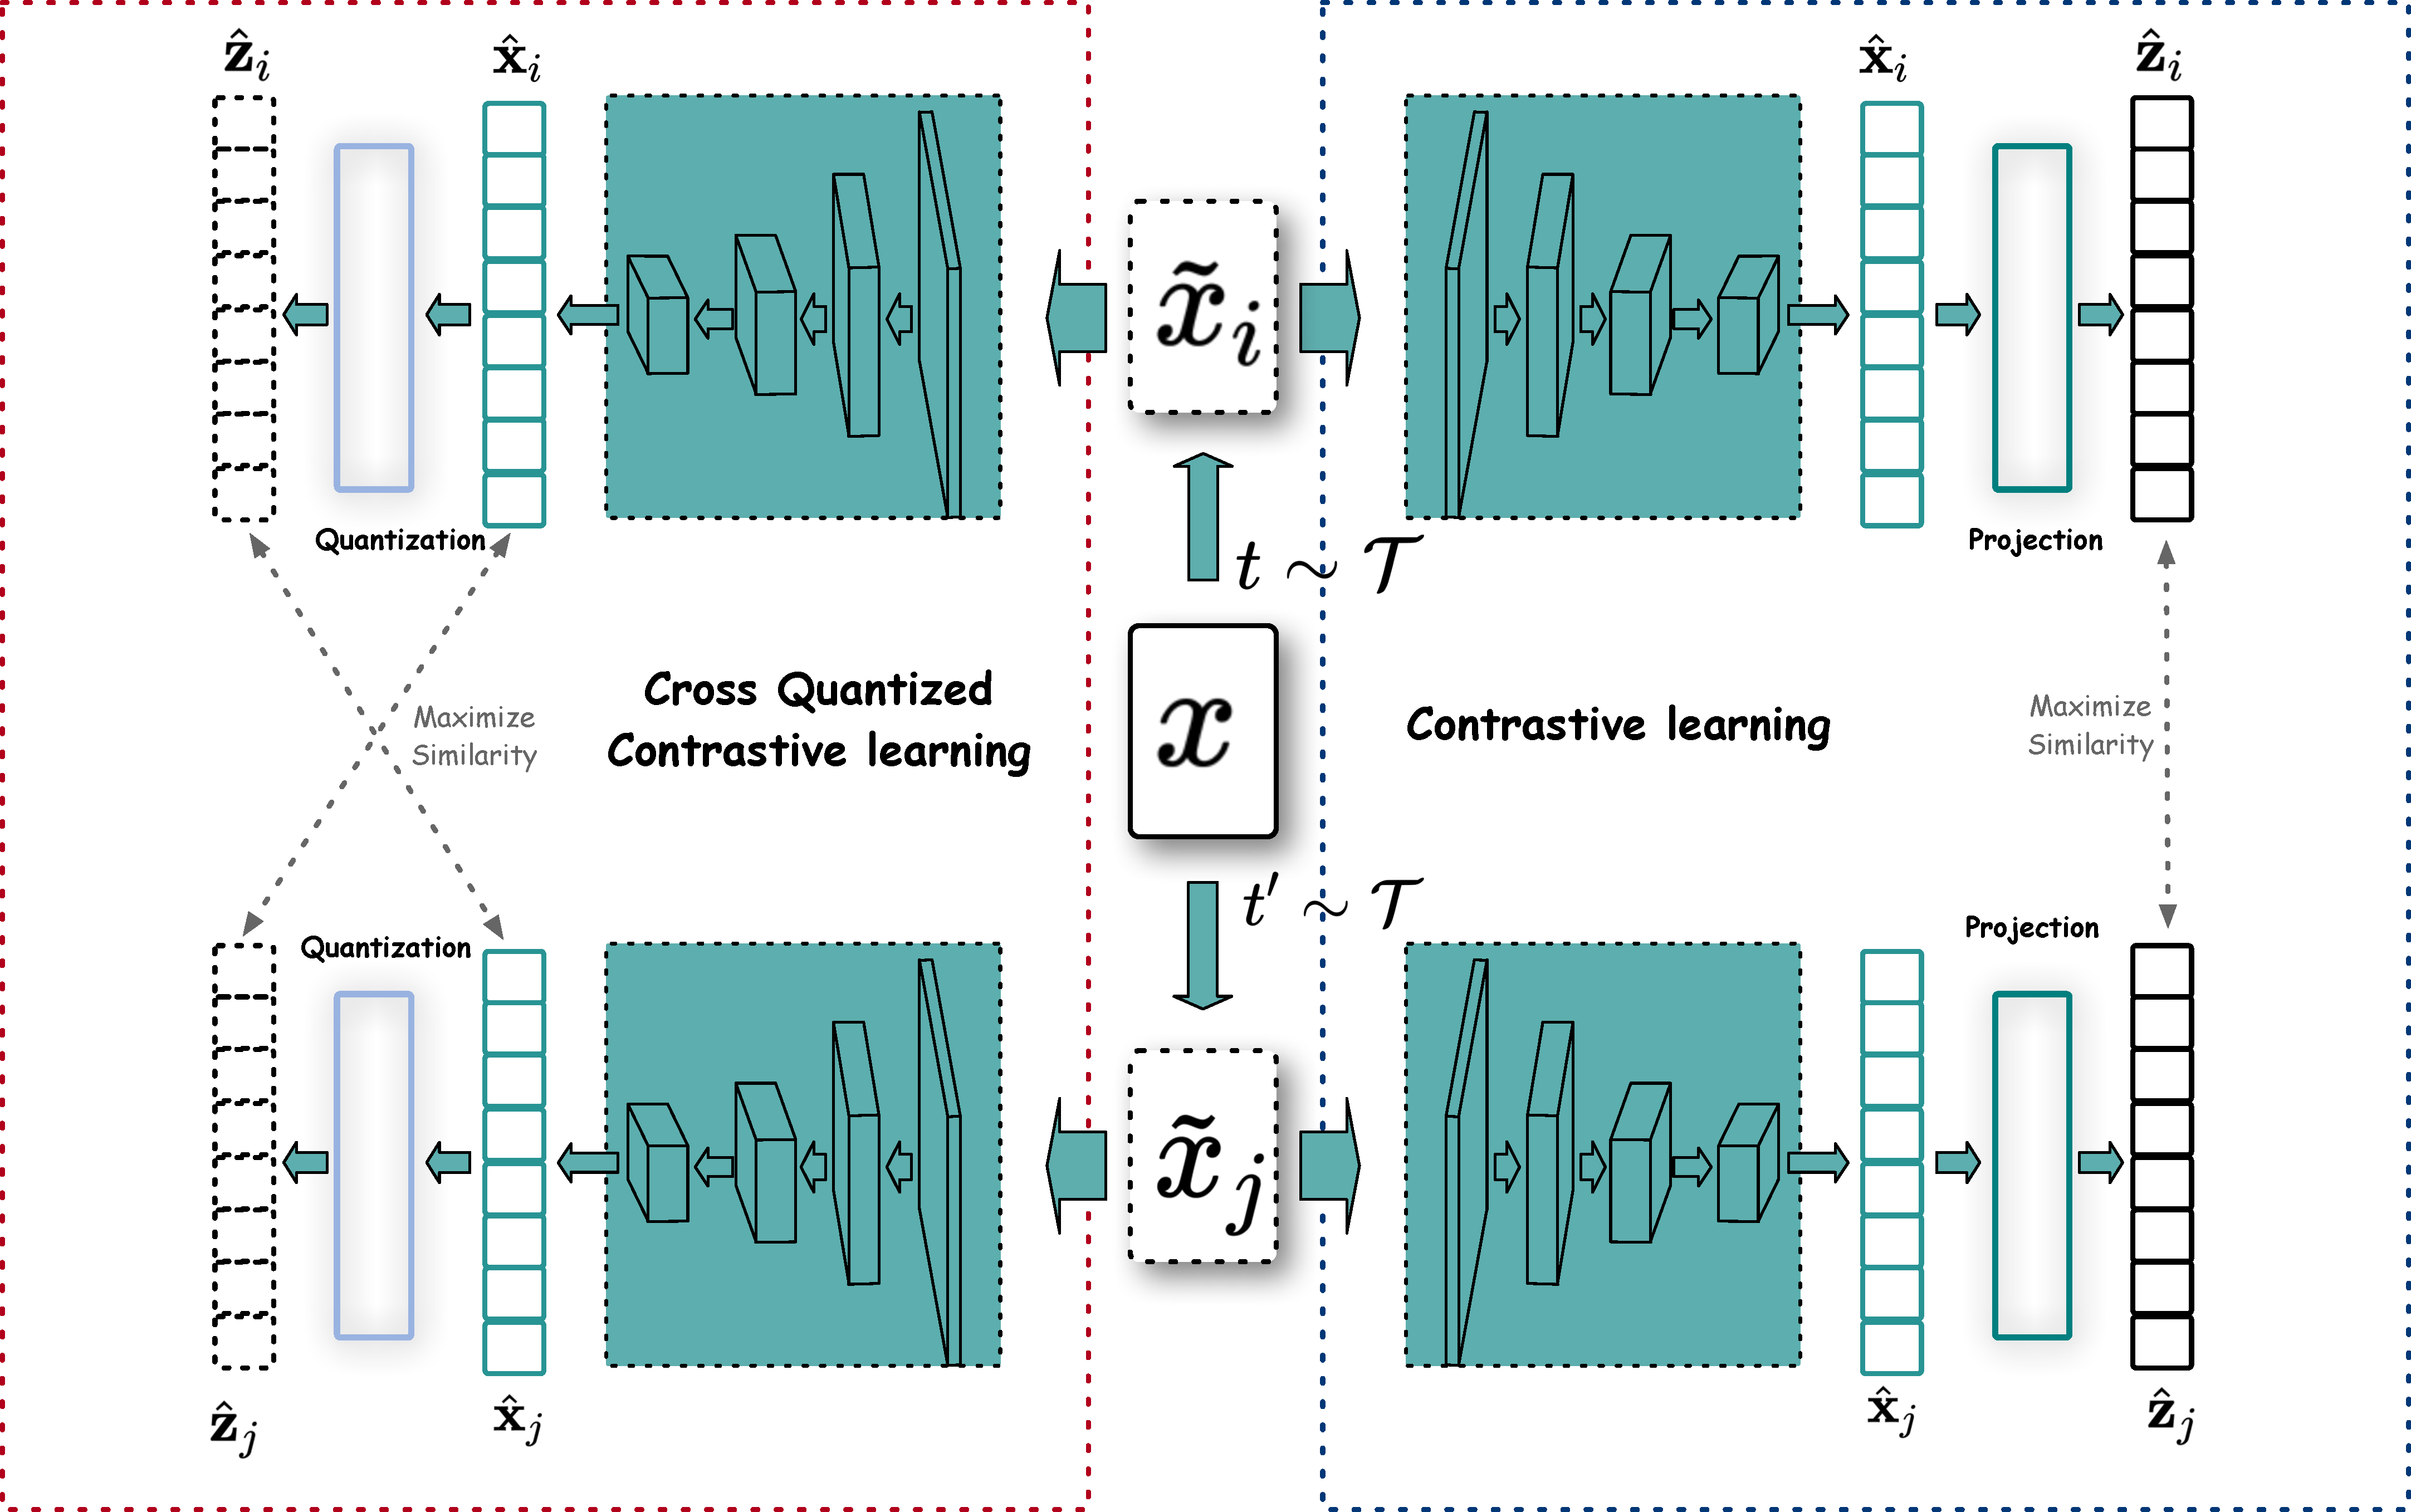
\includegraphics[width=15cm]{spq.pdf} \\
    \bicaption[无监督乘积量化的框架图]
      {右侧是传统的对比学习的框架, 左侧是跨量化的对比学习框架。对于输入的图片$x$, 两个不同的变换函数 $(t, t^{\prime} \sim \mathcal{T})$ 将此图片变换成 $\tilde{x}_i$ 和 $\tilde{x}_j$。传统的对比学习通过一个映射例如全连接将深度描述符$\mathbf{x}$映射到$\mathbf{z}$, 然后在$\mathbf{z}$上进行对比学习。而跨量化的框架使用一个可导的量化层将$\mathbf{x}$映射到$\mathbf{z}$, 同时对比学习是在$\mathbf{x}$和$\mathbf{z}$中进行。}
      {The right is the traditional contrastive learning framework. The left is the cross quantized contrastive learning framework for unsupervised image retrieval. On the right diagram, the projection head outputs $\mathbf{z}$ from the deep descriptor $\mathbf{x}$ and contrastive learning is conducted by comparing the similarity between projection outputs. On the left, the contrastive learning process is conducted between the deep descriptor $\mathbf{x}$ and the output from the quantization head $\mathbf{z}$.}
   \label{fig:spq}
\end{figure}


\begin{equation}
    L_t=\sum_{\mathbf{x}^a}\left[\mathcal{D}\left(\hat{q}\left(\mathbf{x}^a\right), \hat{q}\left(\mathbf{x}^p\right)\right)-\mathcal{D}\left(\hat{q}\left(\mathbf{x}^a\right), \hat{q}\left(\mathbf{x}^n\right)\right)+\alpha\right]_{+}.
\end{equation}
其中, $\mathcal{D}$是欧式距离, $\mathbf{x}^a$ 是anchor图片, $\mathbf{x}^p$是anchor的正样本,  $\mathbf{x}^n$是负样本照片。 \par

2020年, Jang 等人提出 \textbf{SPQ}, 一个完全无监督的乘积量化网络来进行图像检索。如图~\ref{fig:spq}。作者采取对比学习将每张图片随机增强生成两张图片, 这两张图片当成一次训练中的正样本对, 图片和其他图片均视作负样本对。文中提出一个新的乘积量化损失函数:
\begin{equation}
    \ell_{(i, j)}=-\log \frac{\exp \left(\mathcal{S}(i, j) / \tau_{c q c}\right)}{\sum_{n=1}^{N_B} \mathbb{1}_{\left[n^{\prime} \neq j\right]} \exp \left(\mathcal{S}\left(i, n^{\prime}\right) / \tau_{c q c}\right)}.
\end{equation}
其中$\mathcal{S}(i, j)$ 是$\mathbf{\hat{x}}_i$和$\mathbf{\hat{z}}_j$的余弦相似度。$\mathbf{\hat{x}}_i$ 是未经过量化层量化的特征而$\mathbf{\hat{z}}_j$是经过乘积量化后的特征。$\tau_{c q c}$是一个温度超参数。$\mathbb{1}_{\left[n^{\prime} \neq j\right]} \in\{0,1\}$ 是一个示性函数, 当$n^{\prime} \neq j$的时候函数取值为 $1$。


\section{本文章节安排与研究内容}
\subsection{主要研究内容}
如本章前文所述, 图像检索是计算机视觉以及多媒体检索领域一个核心的研究问题, 由于其在电商搜索, 智能安防, 智能医疗等众多领域的广泛应用而获得了国内外学者的广泛的关注。随着自媒体社交网络,计算机硬件,手机数码摄像技术等的发展, 图像数据库的数据总量也以爆炸性的速度急剧增长。为了满足大规模图像检索对于检索速度以及内存消耗的需求, 基于深度哈希的图像检索成为主流方法。本文主要研究了基于深度哈希以及量化的图像检索方法, 探究其在行人重识别, 车辆重识别的应用。同时, 受视觉Transformer在图像特征提取以及多个计算机视觉任务领域的优异表现的启发, 本文在通用的深度哈希图像检索领域提出基础网络架构的创新, 以及用于监督的哈希损失的创新, 具有较高的理论意义以及广泛的工业应用价值。本文的主要内容与创新如下: \par

首先, 本文对图像检索的一个典型应用-行人重识别问题进行了深入的探讨。传统的行人重识别问题针对单模态的数据,也就是检索的图片和数据库中的图片来自同一模态。而现实中的监控摄像头一般能同时在日间和夜间工作捕捉不同模态的行人照片,这使得跨模态行人重识别成为计算机视觉领域一个热门的研究课题。由于模态鸿沟的存在(Modality Gap), 跨模态行人重识别比单模态行人重识别更具有挑战性。传统基于双流卷积神经网络的算法,很难学习到模态恒定(Modality-invariant)的特征。针对这一难点,本文创新性的基于自编码器(Autoencoder)设计了一个神经网络架构学习模态恒定以及外表恒定的特征。同时设计了适用于跨模态检索对齐不同模态特征的损失函数,使得网络可以在动态创建的图片对上进行监督训练。我们在标准的跨模态重识别数据集上进行了训练以及测试,结果表明我们的算法可以取得优越的性能数据,证明了算法的有效性。 \par
其次,本文首次将深度哈希引入了大规模车辆检索的研究中。传统基于实值向量检索的车辆重识别算法虽然精度高,但是由于其存储效率低以及检索速度慢,无法适用于真实环境的大规模车辆检索。为了提高车辆检索的速度以及优化存储开销,本文第一个探索了深度哈希在大规模车辆检索中的应用。本文提出一个新型的离散哈希模块,通过同时使用传统的基于困难三元组的损失函数进行特征学习,以及离散哈希模块生成离散的汉明哈希码。为了优化离散的哈希架构,我们提出了一个交替优化算法来进行整个架构的优化。 本文在主流的车辆重识别数据集上进行了四种不同长度哈希码的精度测试,显著的超越了当前的普适的哈希算法。 \par
进一步地, 为了优化深度哈希算法的表征能力,我们第一次探索一个不基于卷积神经神经网络的深度哈希框架。视觉Transformer(Vision Transformer)是一种基于自注意力机制(Self-attention)的新型的计算机视觉基础网络模型。本文提出了第一个完全基于视觉Transformer的深度哈希框架,通过设计一个孪生视觉Transformer架构,以及一个新型的双流特征学习的视觉Transformer模块来进行细粒度表征学习。 同时,我们采取成对的基于贝叶斯的学习框架进行度量学习。本文在三个标准化的图像检索基准数据集上进行测试,实验效果表明该方法可以大幅度提升检索的性能。 \par
最后, 由于基于传统哈希编码的方法会带来较大的精度损失,本文探索一种基于乘积量化(Product Quantization)编码的深度哈希算法来提高检索性能。同时,本文提出第一个基于视觉Transformer的乘积量化神经网络。为了进行细粒度的特征学习,考虑到视觉Transformer的表征能力与采取的图片分块策略紧耦合的特点, 本文设计了一个双支视觉Transformer量化的支柱网络。同时,本文设计了一个基于排序损失的直接优化平均查准率 (Average Precision)的量化损失函数来进行度量学习。文章将乘积量化集成到端到端的神经网络优化中,取得了优异的性能表现。

\subsection{本文的组织结构}
本文一共分为六个章节。结构如下: \par
第一章: 首先介绍了研究的主要背景以及研究意义, 同时介绍了大规模图像检索面临的挑战。随后主要介绍了图像检索的发展历史以及国内外的研究现状, 主要讲述了早期基于手工特征的图像检索, 以及深度学习的主干网络进展现状, 之后介绍了基于深度特征的图像检索,最后着重阐述基于深度哈希的检索方法的背景以及各种最新的研究技术。本章最后介绍文章的主要结构以及贡献。 \par
第二章: 对图像检索的经典应用跨模态行人重识别问题进行了深入研究。设计了一个 MAENet 网络来对齐两个模态的特征, 并且设计了新型的跨模态检索的损失函数来进行监督训练, 在两个标准的跨模态重识别数据集上进行训练和测试证明了算法的有效性。 \par
第三章: 第一次将深度哈希技术应用到车辆重识别领域, 设计一个新型的离散哈希模块, 架构可以同时通过基于困难三元组的损失函数进行特征学习, 以及离散的哈希模块来生成汉明哈希码, 实验证明该方法可以大幅度提升大规模车辆检索的性能。 \par
第四章: 提出第一个基于视觉Transformer的深度哈希架构, 通过基于孪生视觉Transformer以及一个新型的双流特征学习模块, 和基于贝叶斯学习的框架来进行细粒度表征学习。在标准化的图像检索数据集上取得了显著的性能提升。 \par
第五章: 提出了一种第一个基于乘积量化的视觉Transformer用于大规模图像检索。设计了一个双支视觉Transformer 量化网络, 同时设计了一个基于排序损失的量化损失函数来直接进行量化编码学习, 在多个数据集上验证了该算法的效果。 \par
第六章: 对本文的主要创新点与研究内容进行了总结, 并对未来的研究进行展望。 \par 
本文的组织结构图如图~\ref{fig:overallarch}所示。
\begin{figure}[!htp]
    \centering
    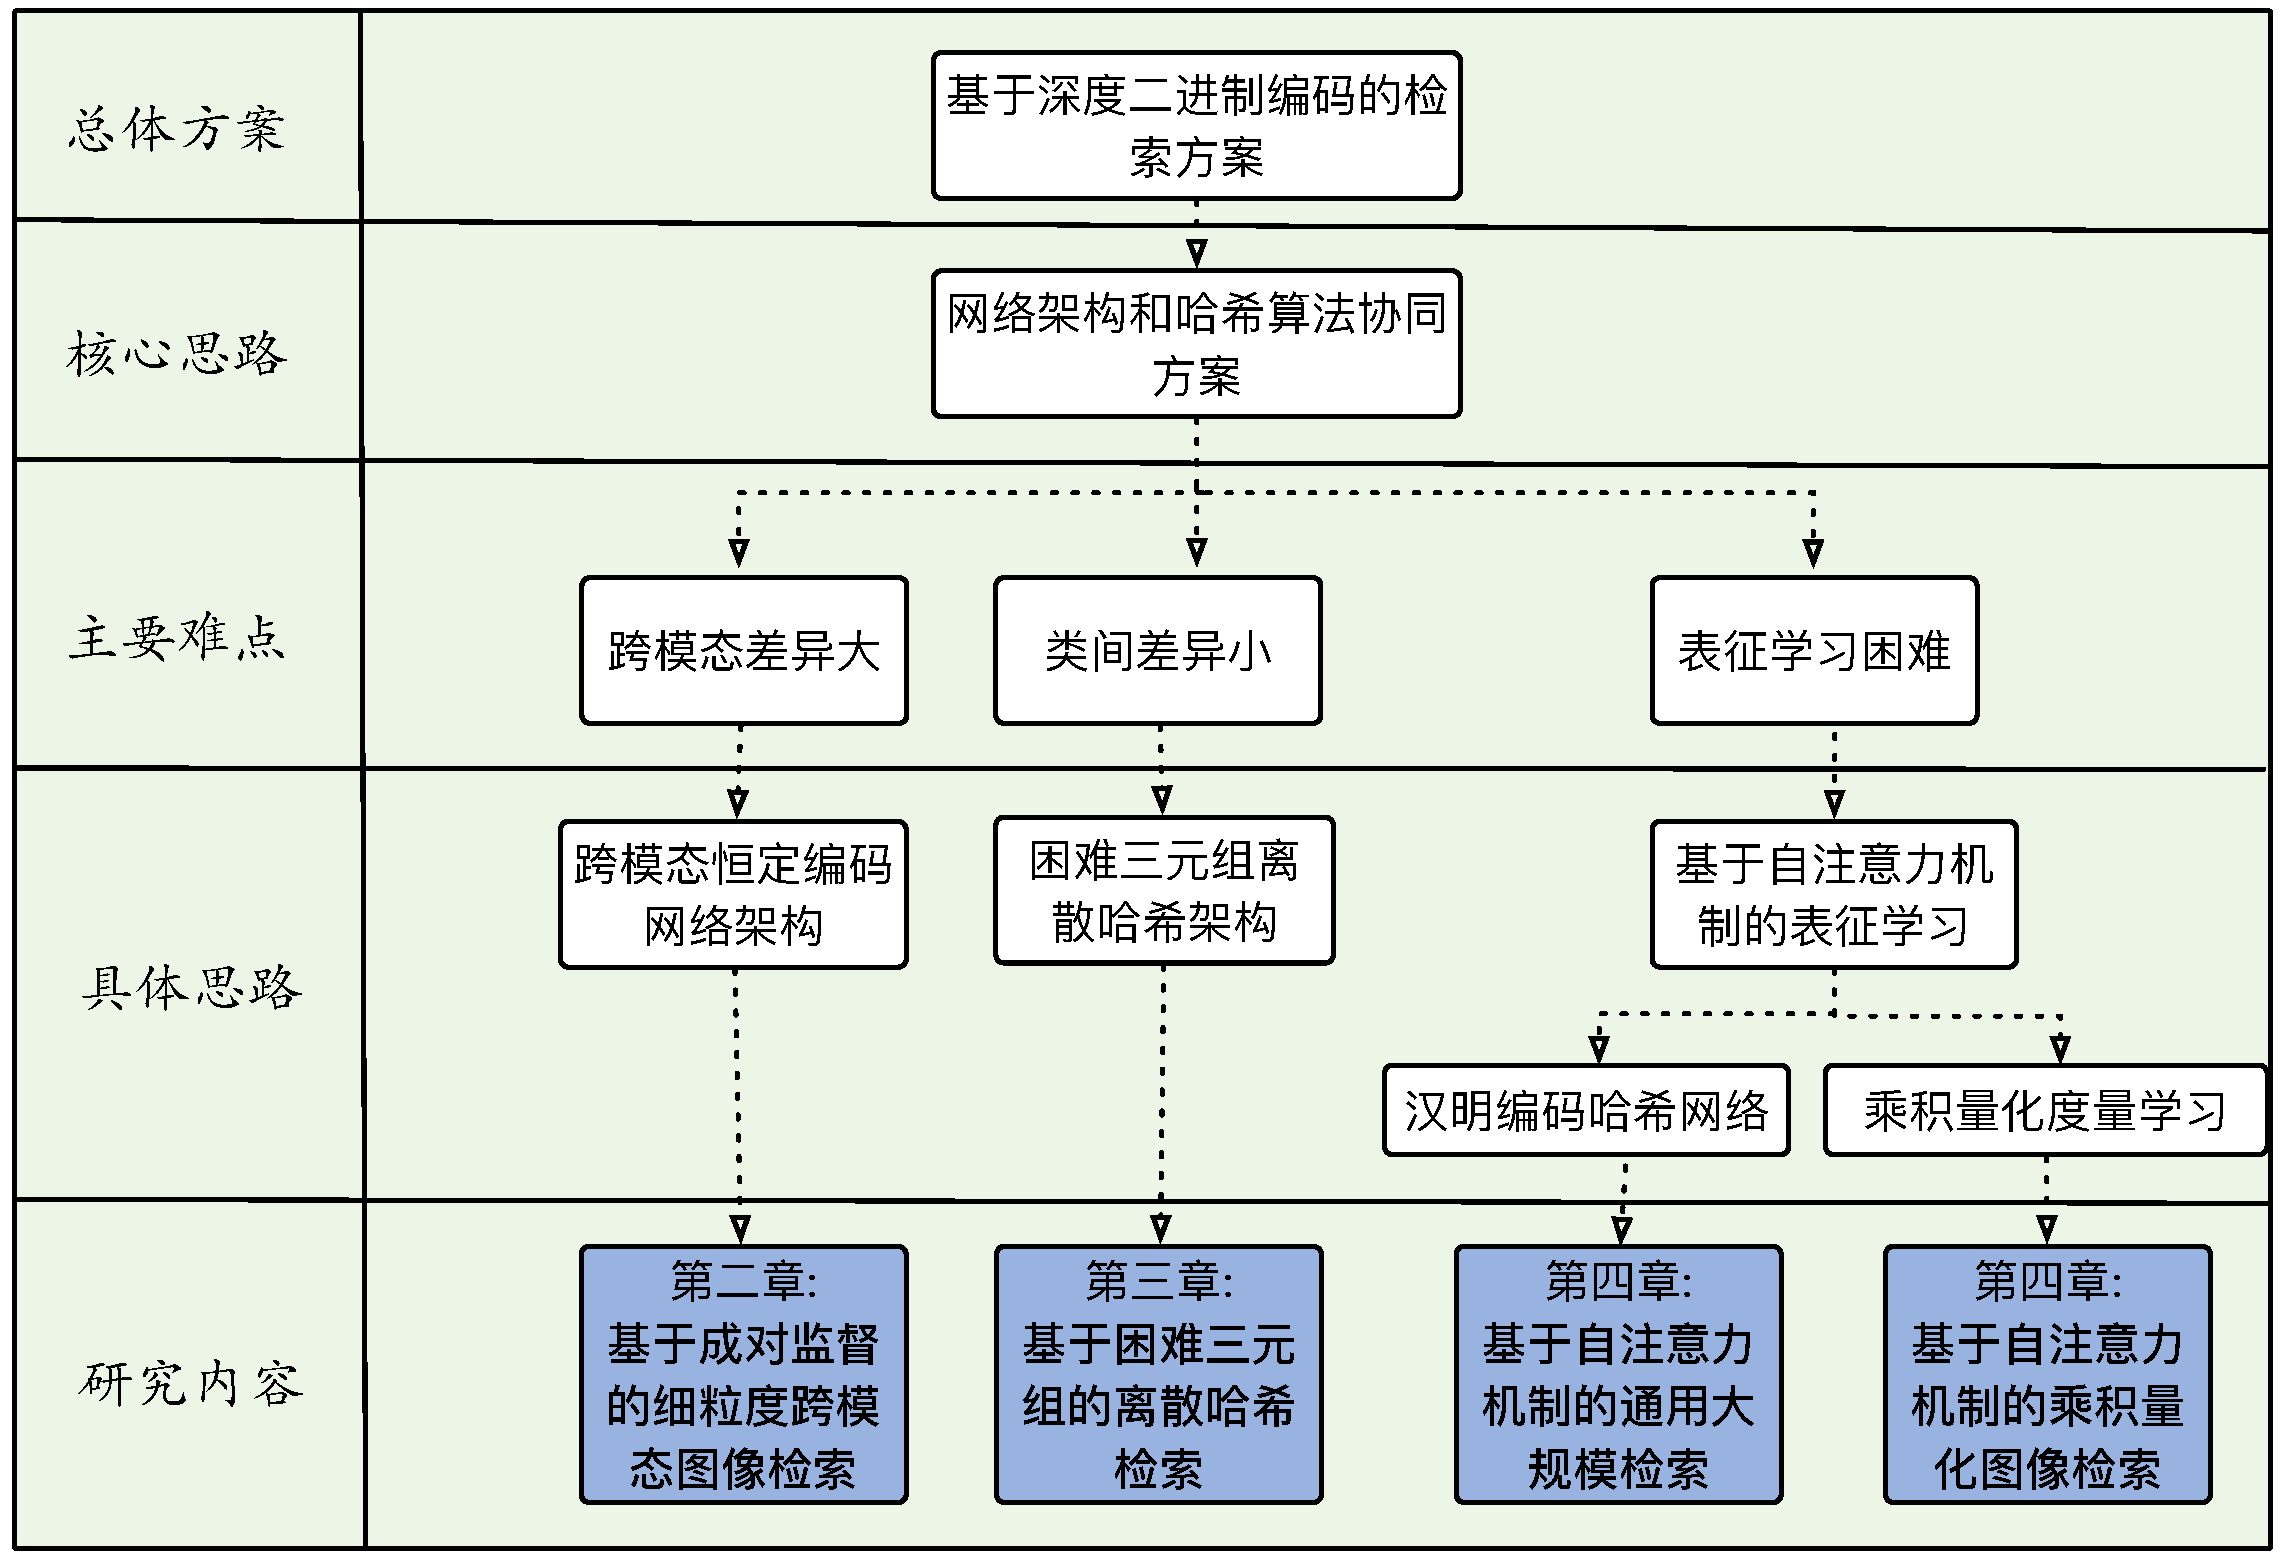
\includegraphics[width=14cm]{paper_arch.pdf} \\
    \bicaption[文章组织结构图]
      {文章的组织结构图}
      {The architecture of this thesis.}
   \label{fig:overallarch}
\end{figure}